\clearpage
\chapter{Grundgedanke des Spiels}
\section{Unternehmensbeschreibung}

\section{Fachkonzept}
\section{Mockup/UI}
Das MockUp für die 1. Iteration wie auch das finale UI wurde auf Basis von HTML und Bootstrap erstellt. 
\subsection{Mockup}
\begin{figure} [h]
	\centering
	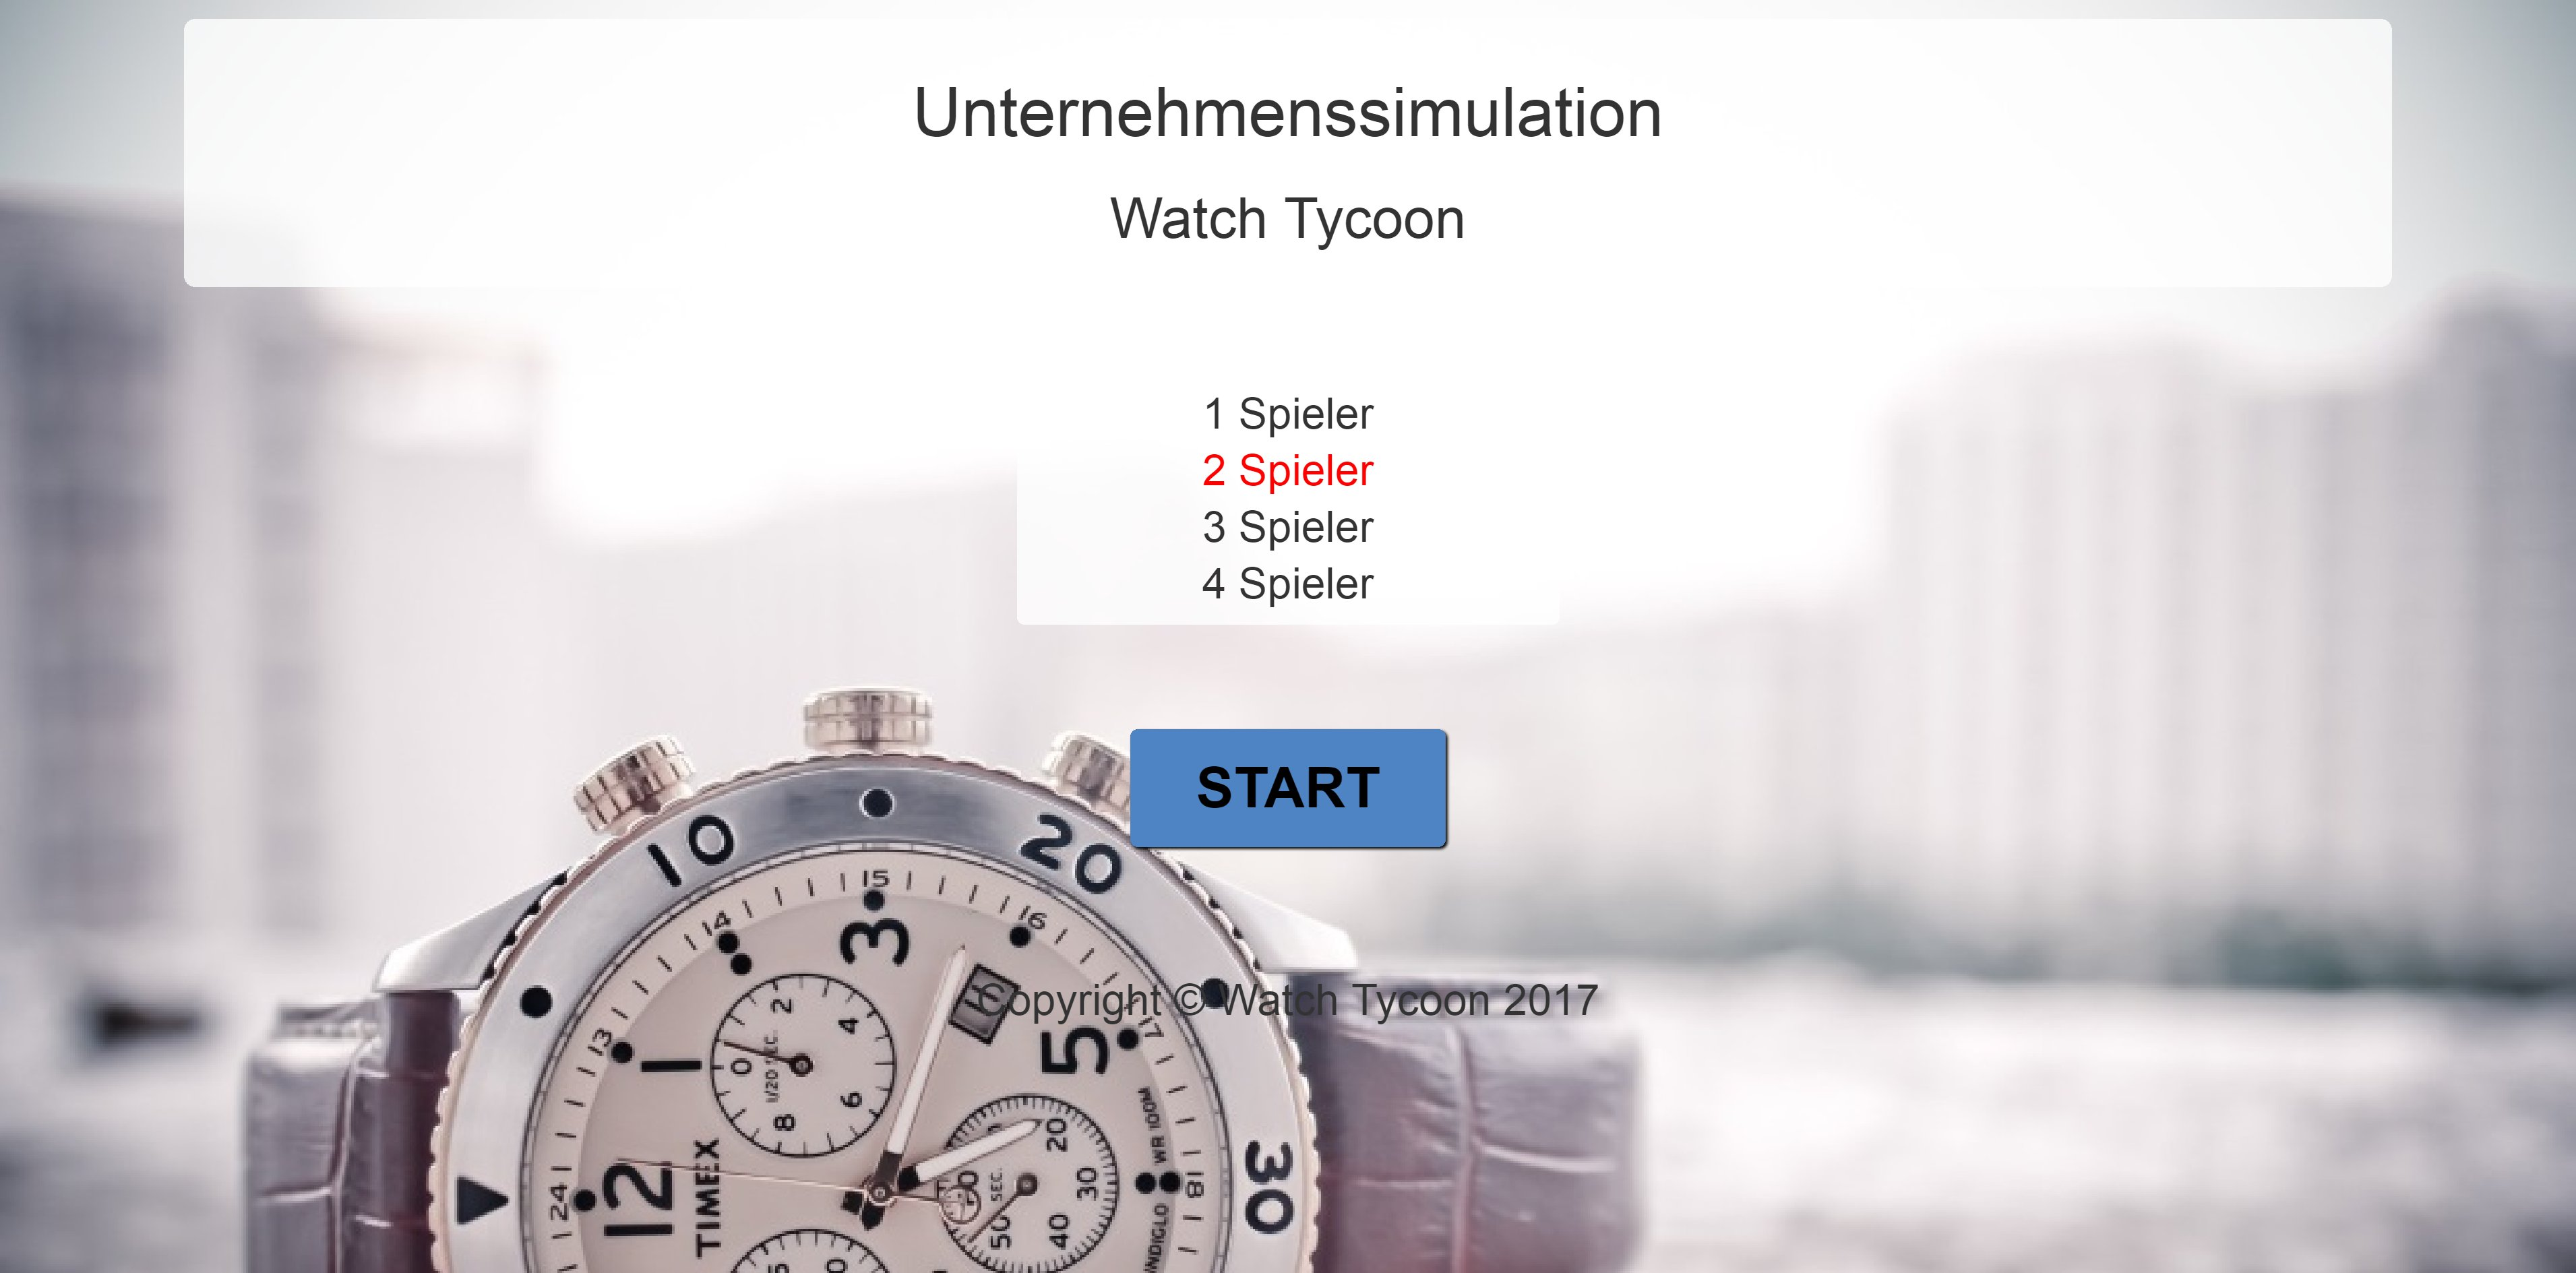
\includegraphics[scale=0.1]{img/bilder_layout/MockUp1.jpg} 
\end{figure}
\begin{figure} [h]
	\centering
	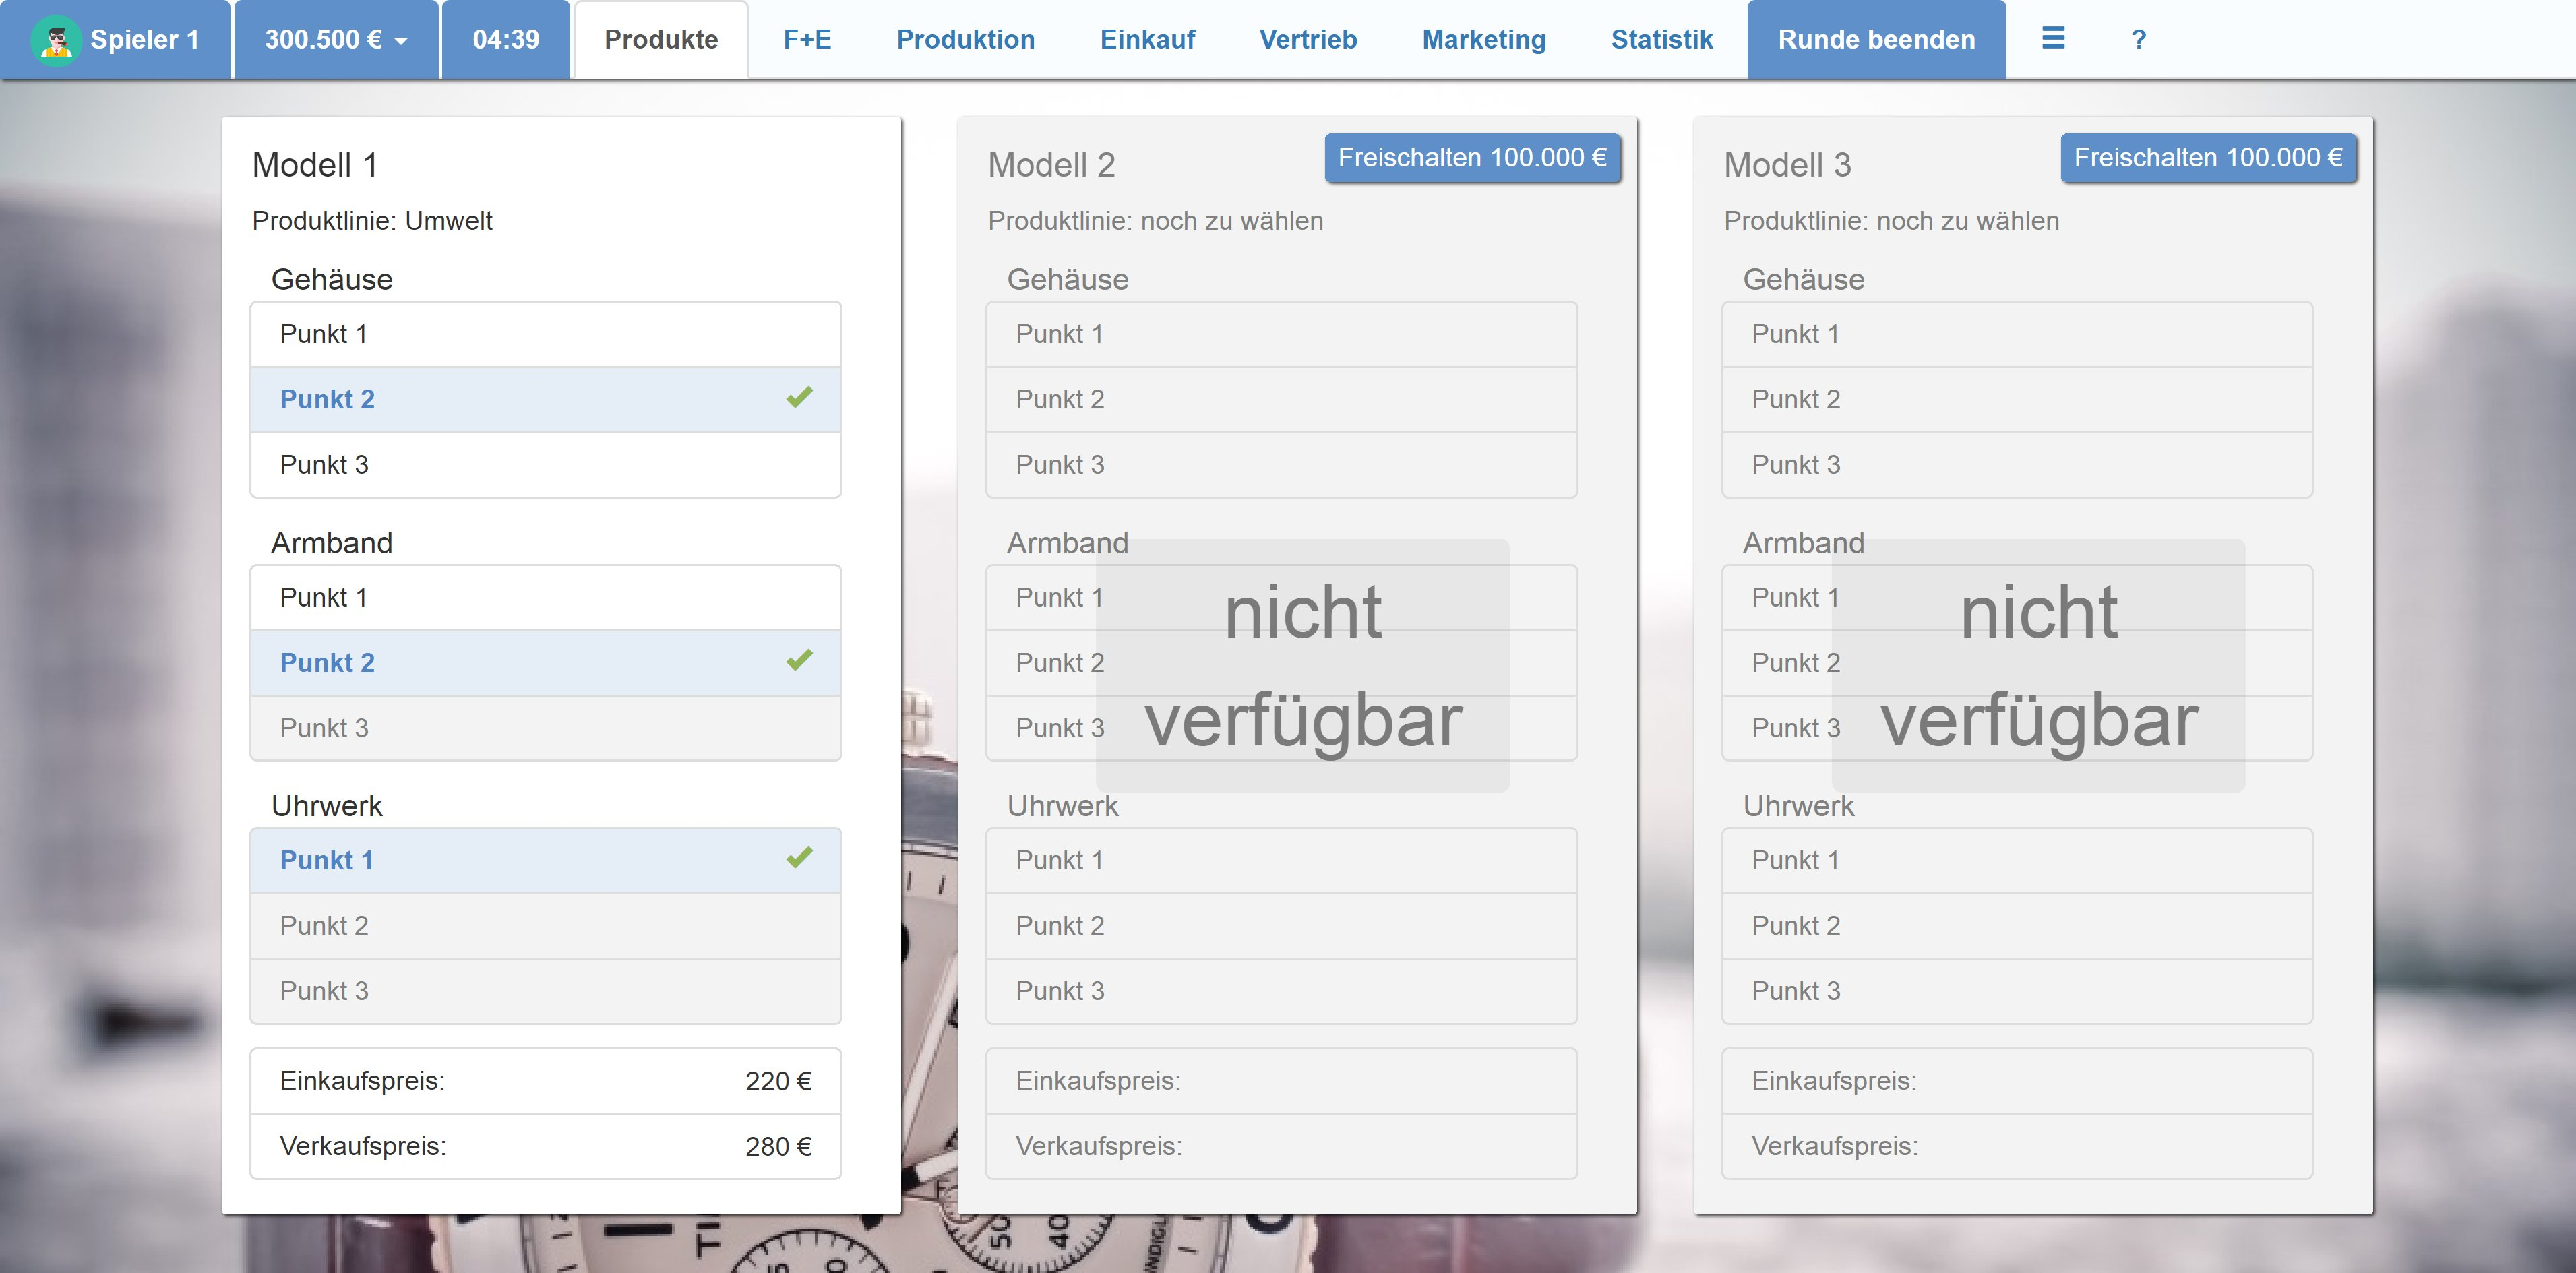
\includegraphics[scale=0.1]{img/bilder_layout/MockUp2.jpg} 
\end{figure}
\begin{figure} 
	\centering
	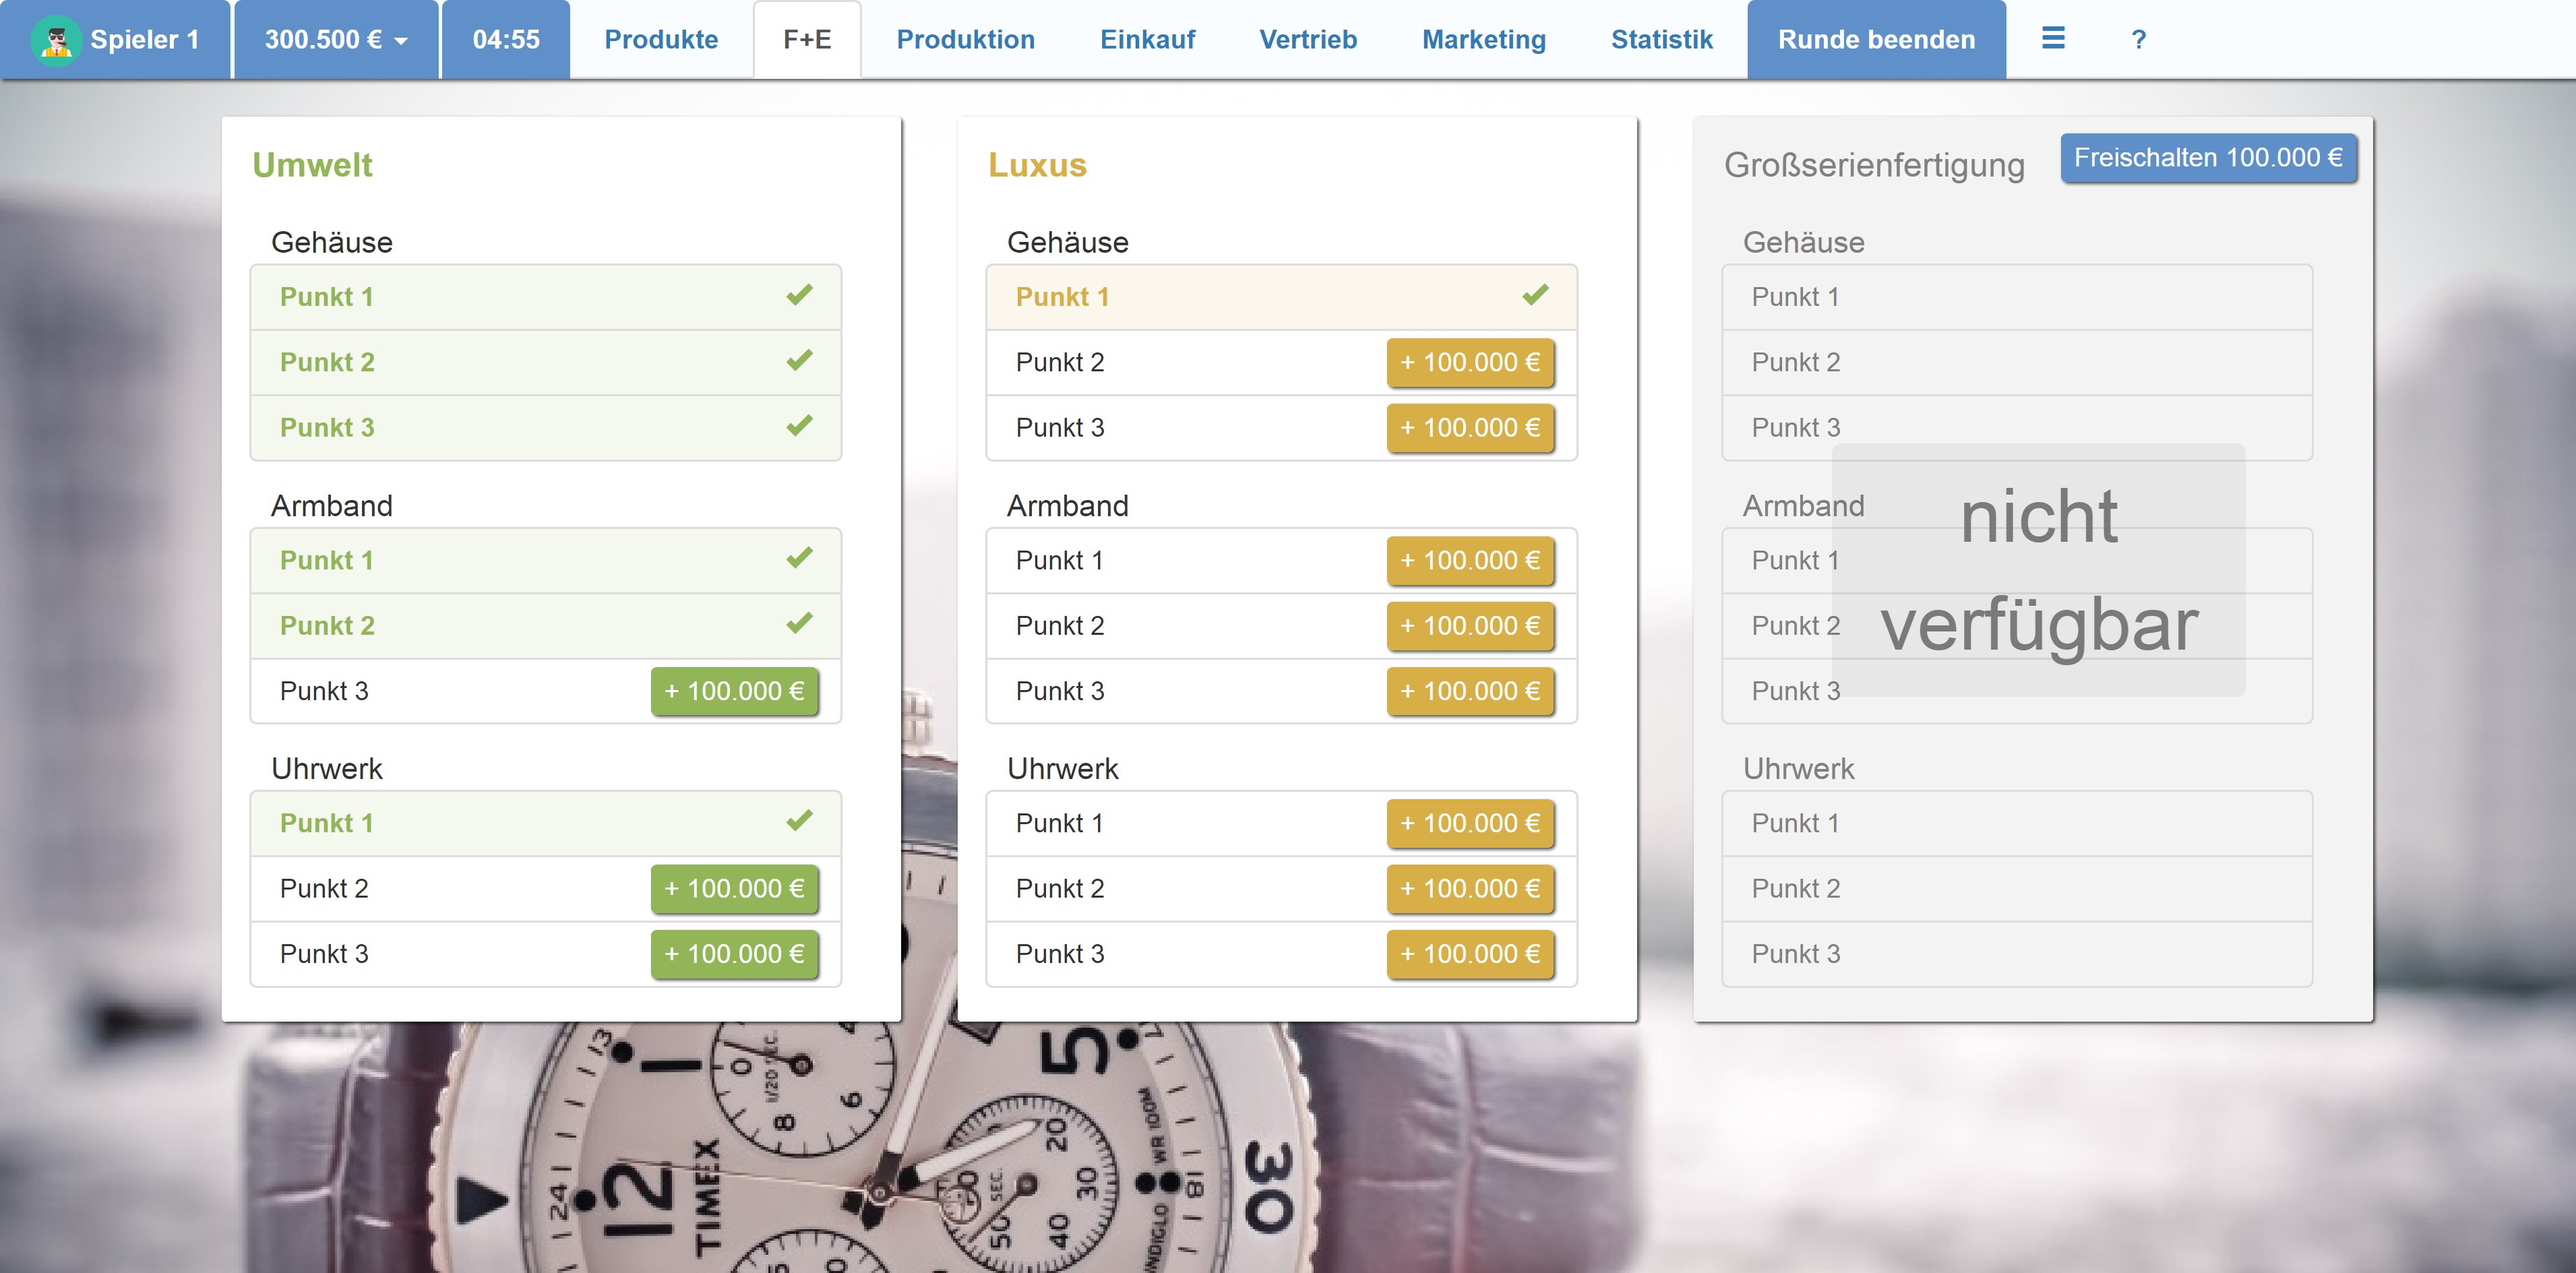
\includegraphics[scale=0.1]{img/bilder_layout/MockUp3.jpg} 
\end{figure}
\begin{figure} 
	\centering
	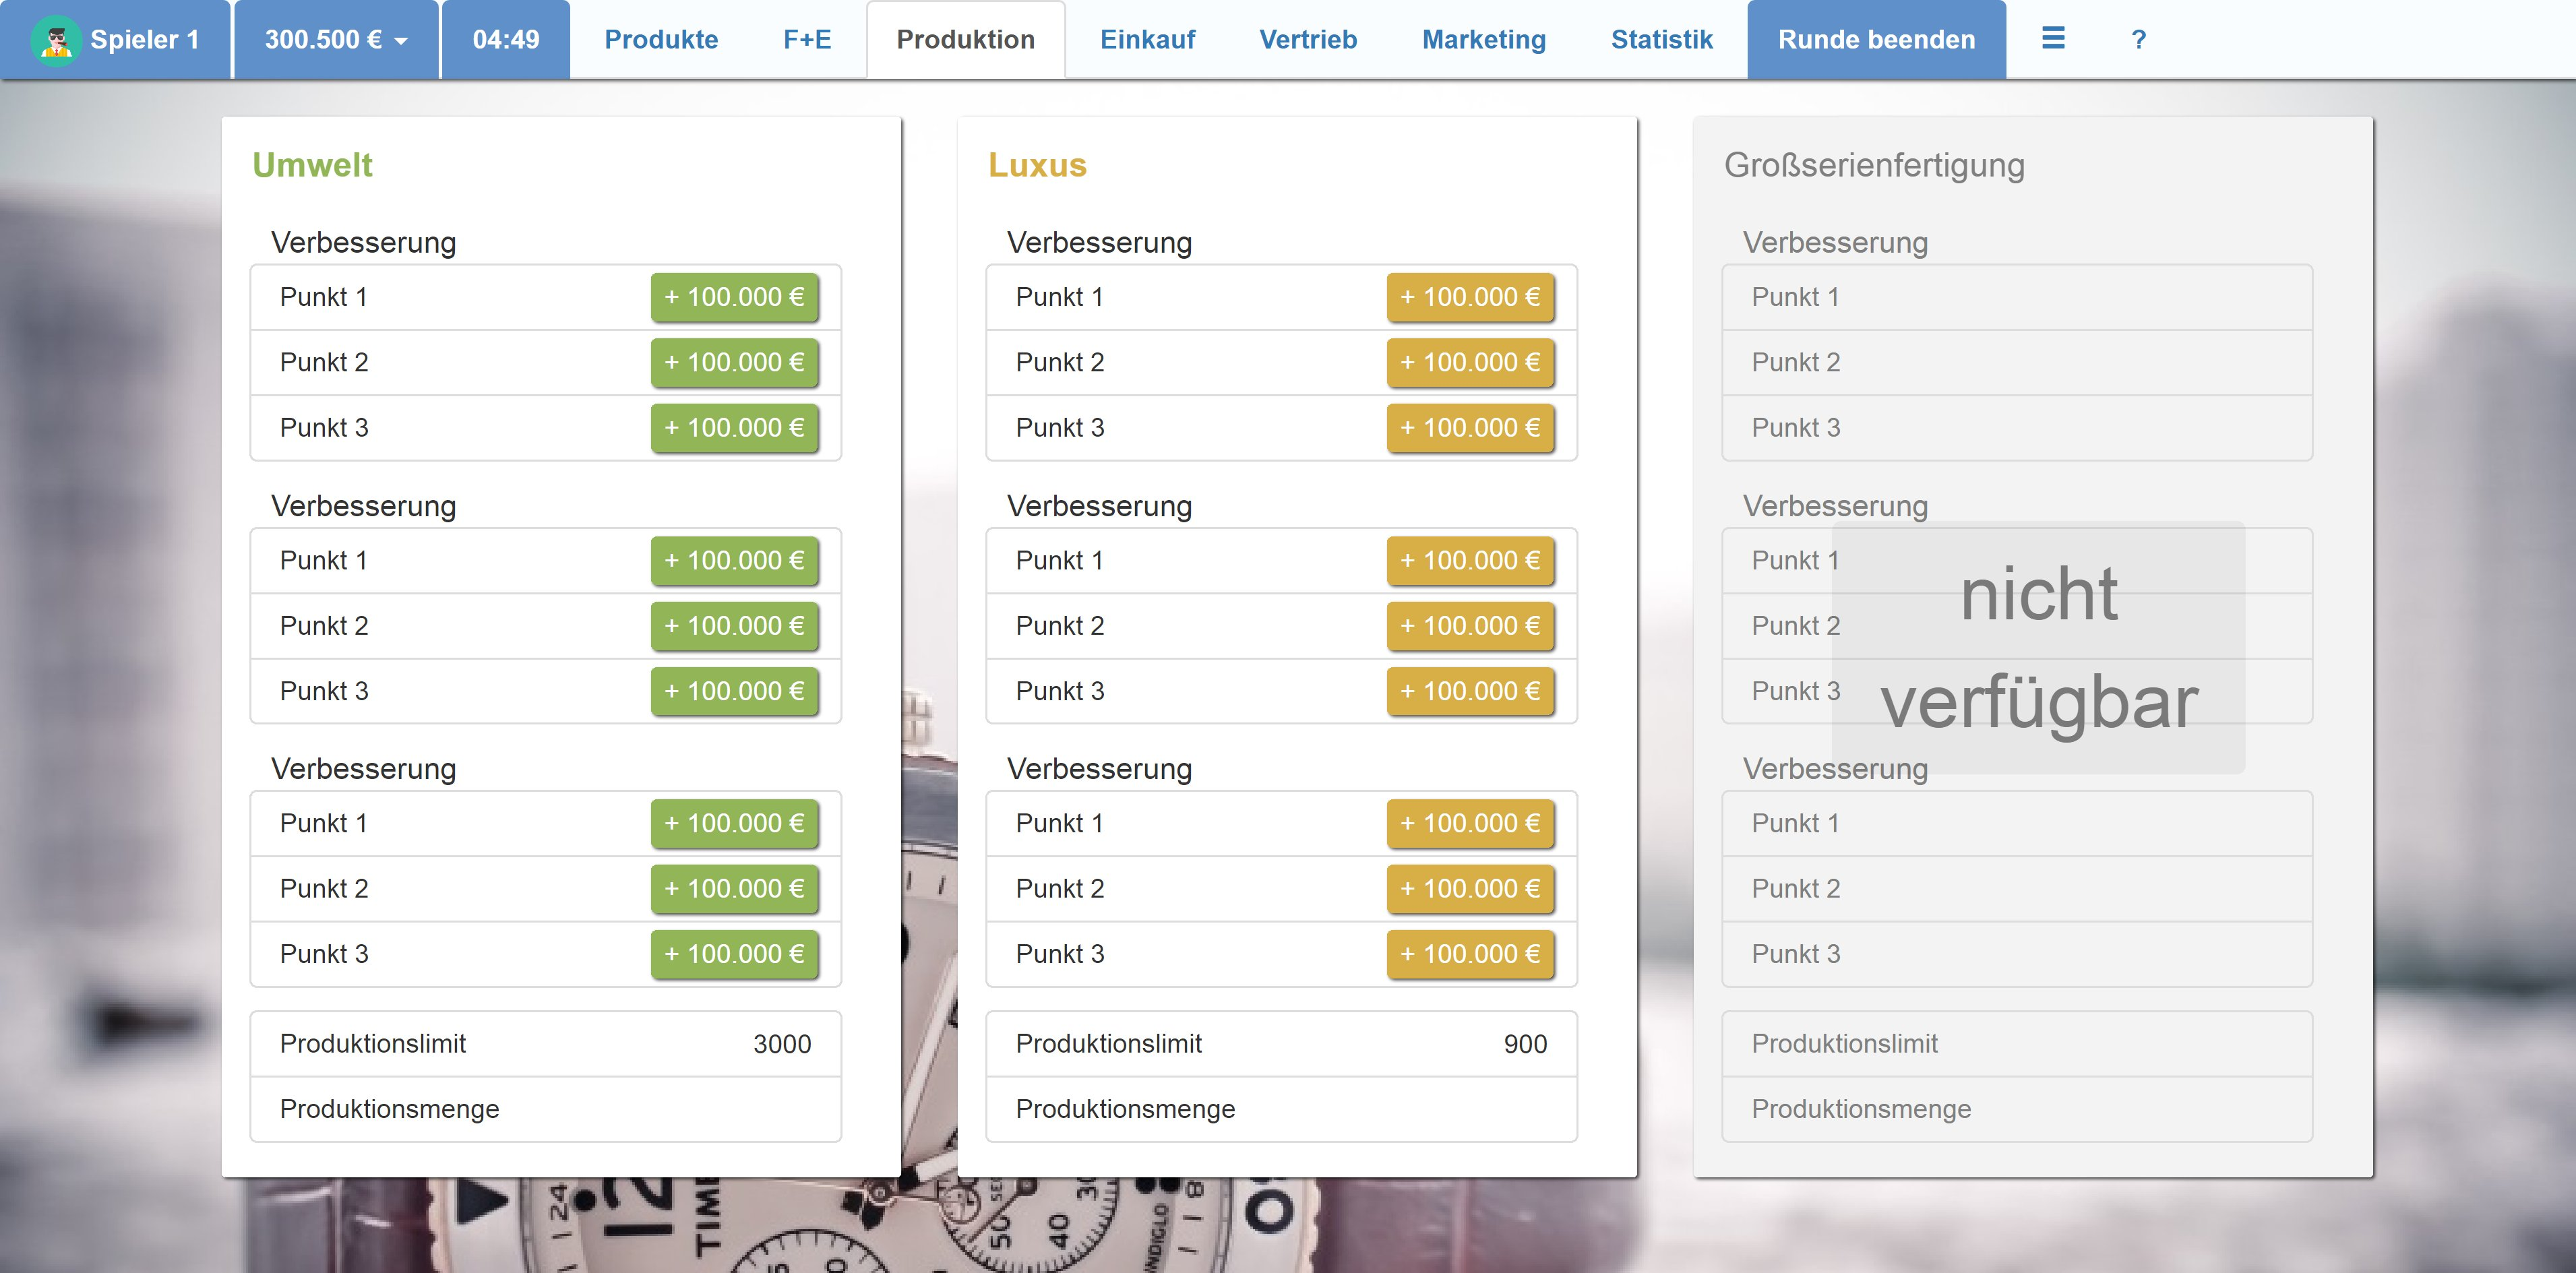
\includegraphics[scale=0.1]{img/bilder_layout/MockUp4.jpg} 
\end{figure}
\begin{figure} 
	\centering
	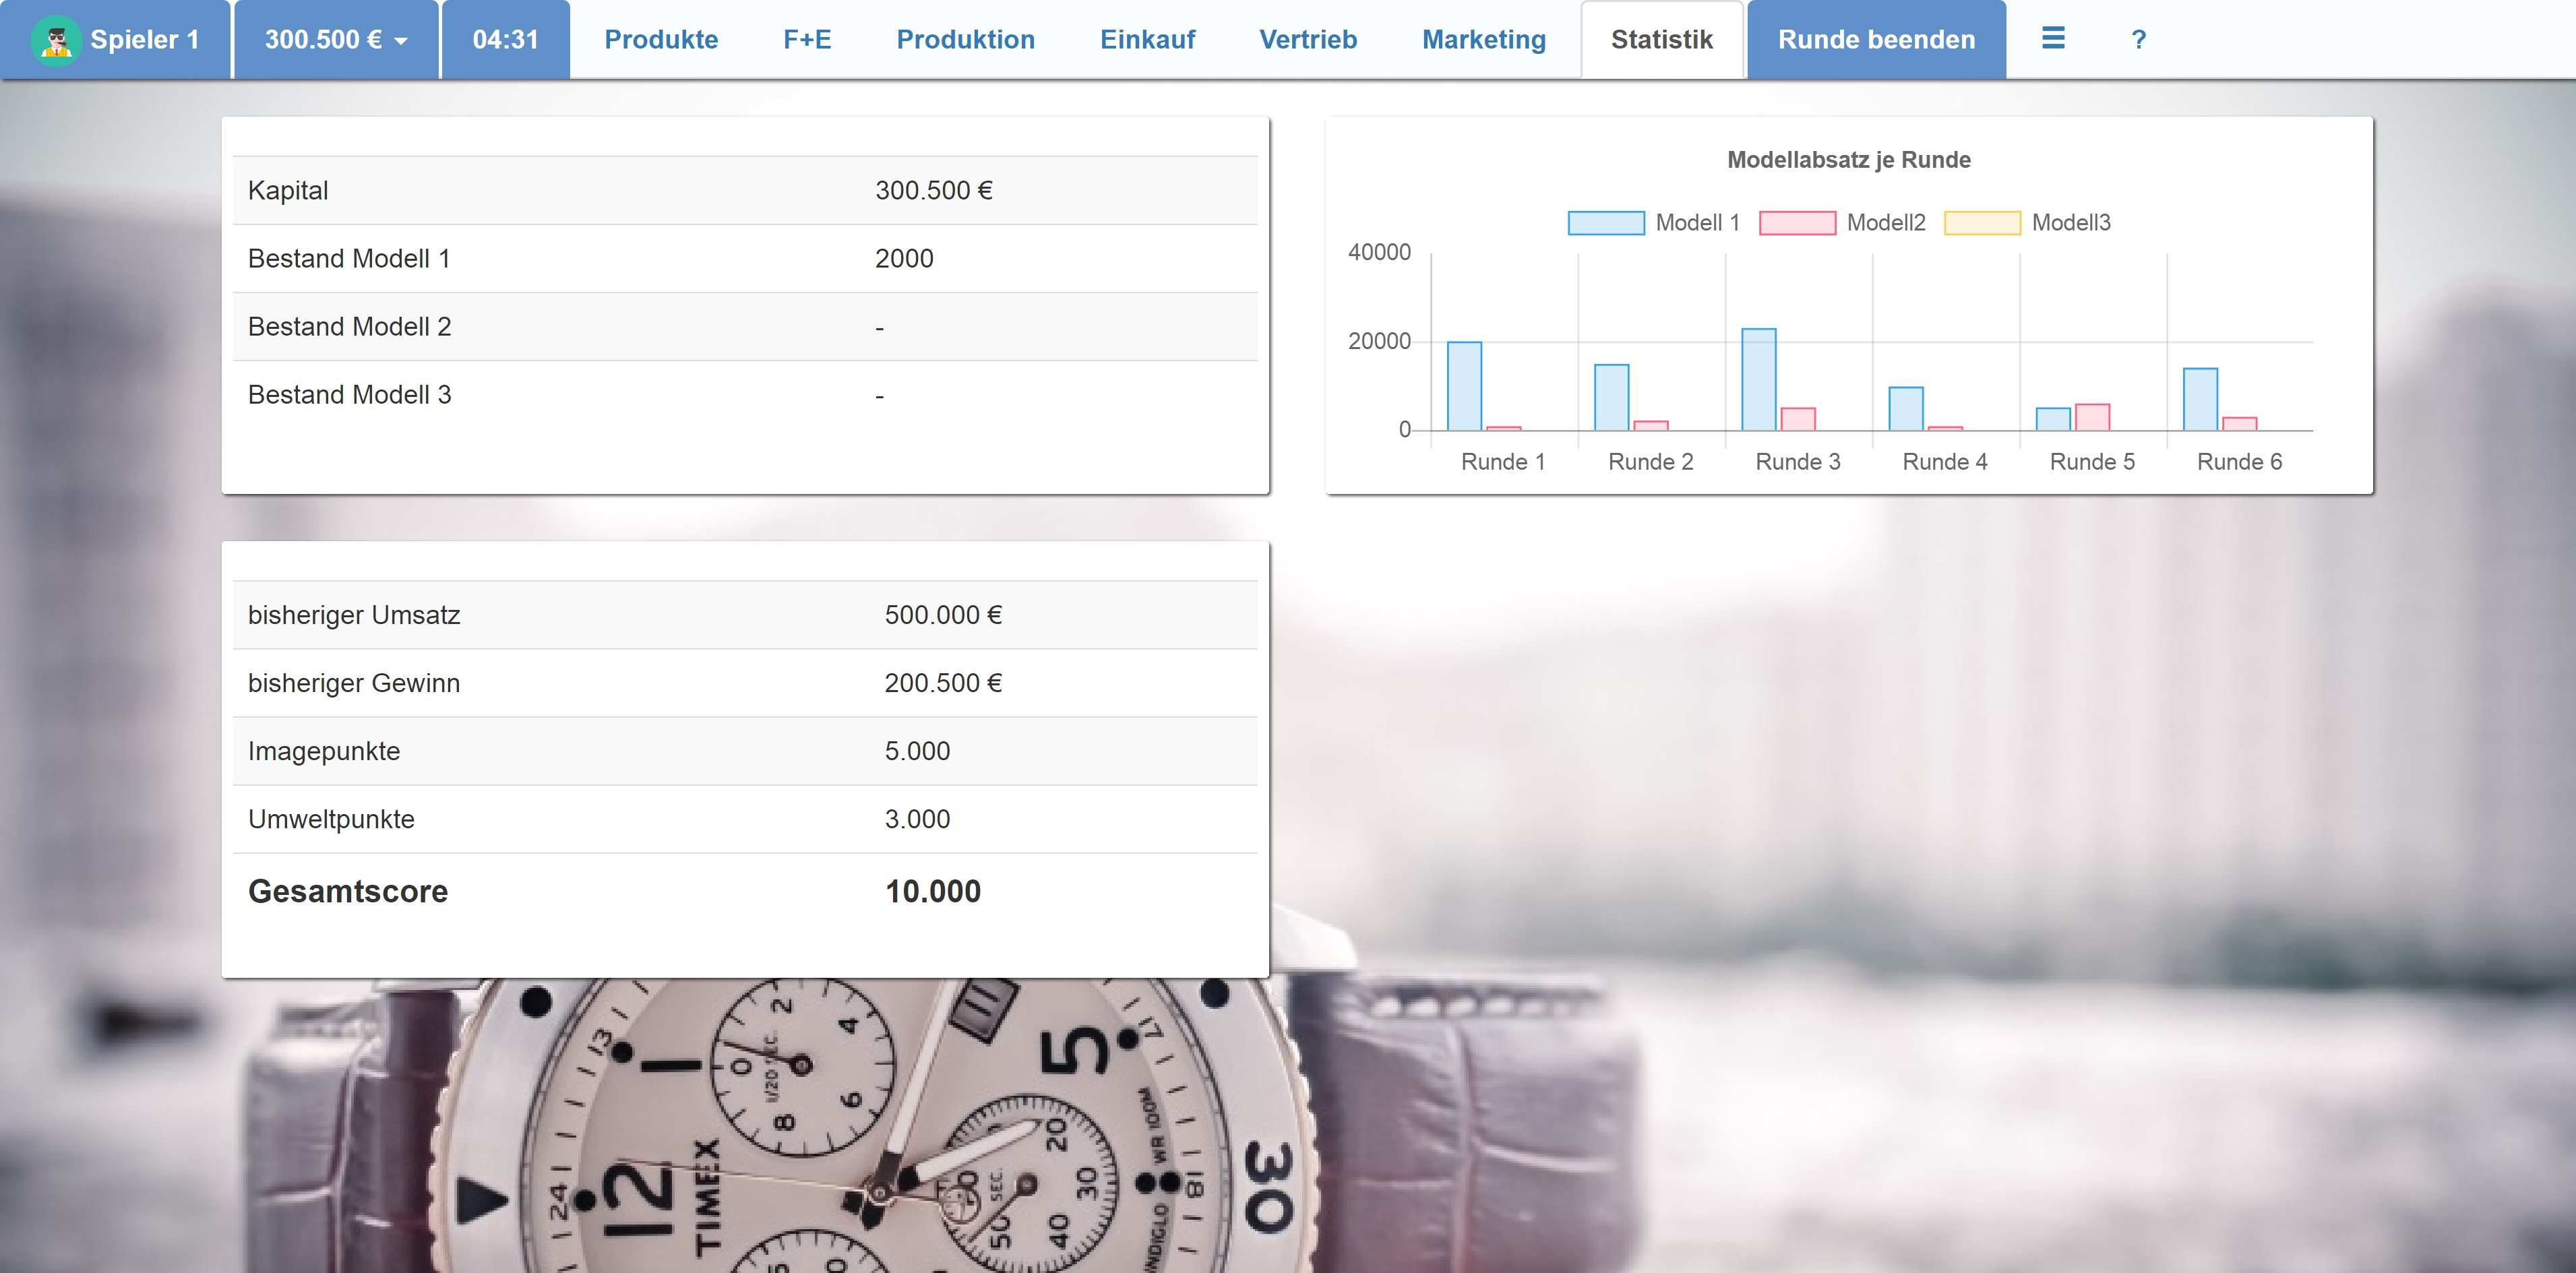
\includegraphics[scale=0.1]{img/bilder_layout/MockUp5.jpg} 
\end{figure}
\begin{figure} 
	\centering
	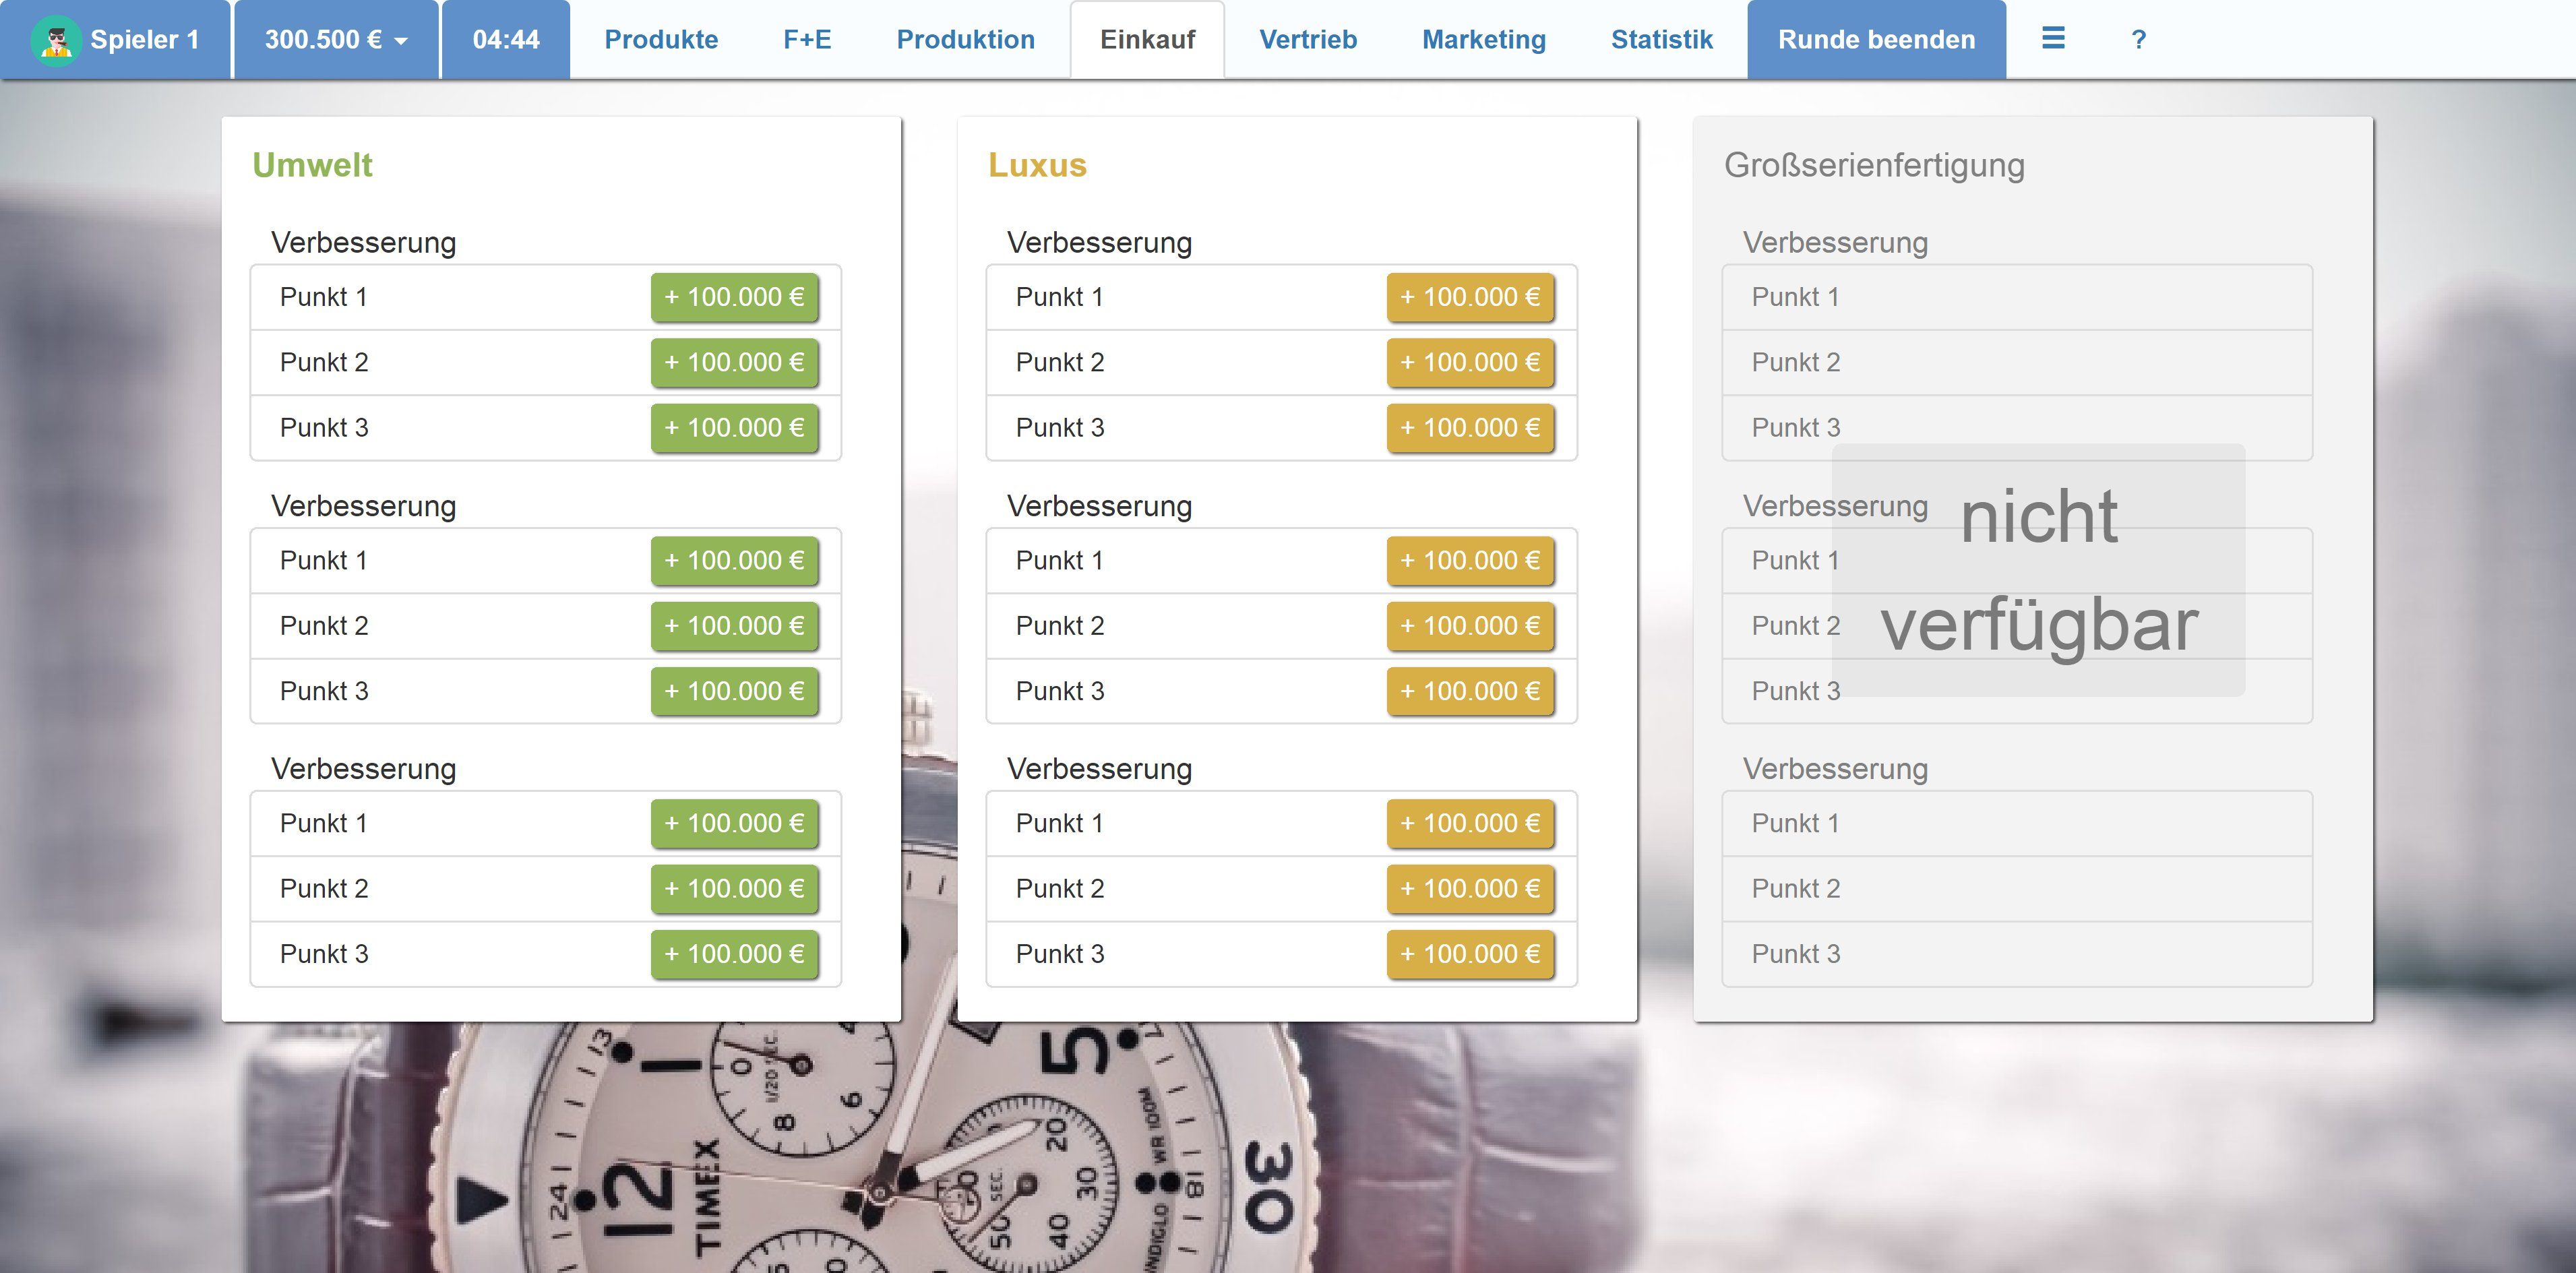
\includegraphics[scale=0.1]{img/bilder_layout/MockUp6.jpg} 
\end{figure}
\begin{figure} 
	\centering
	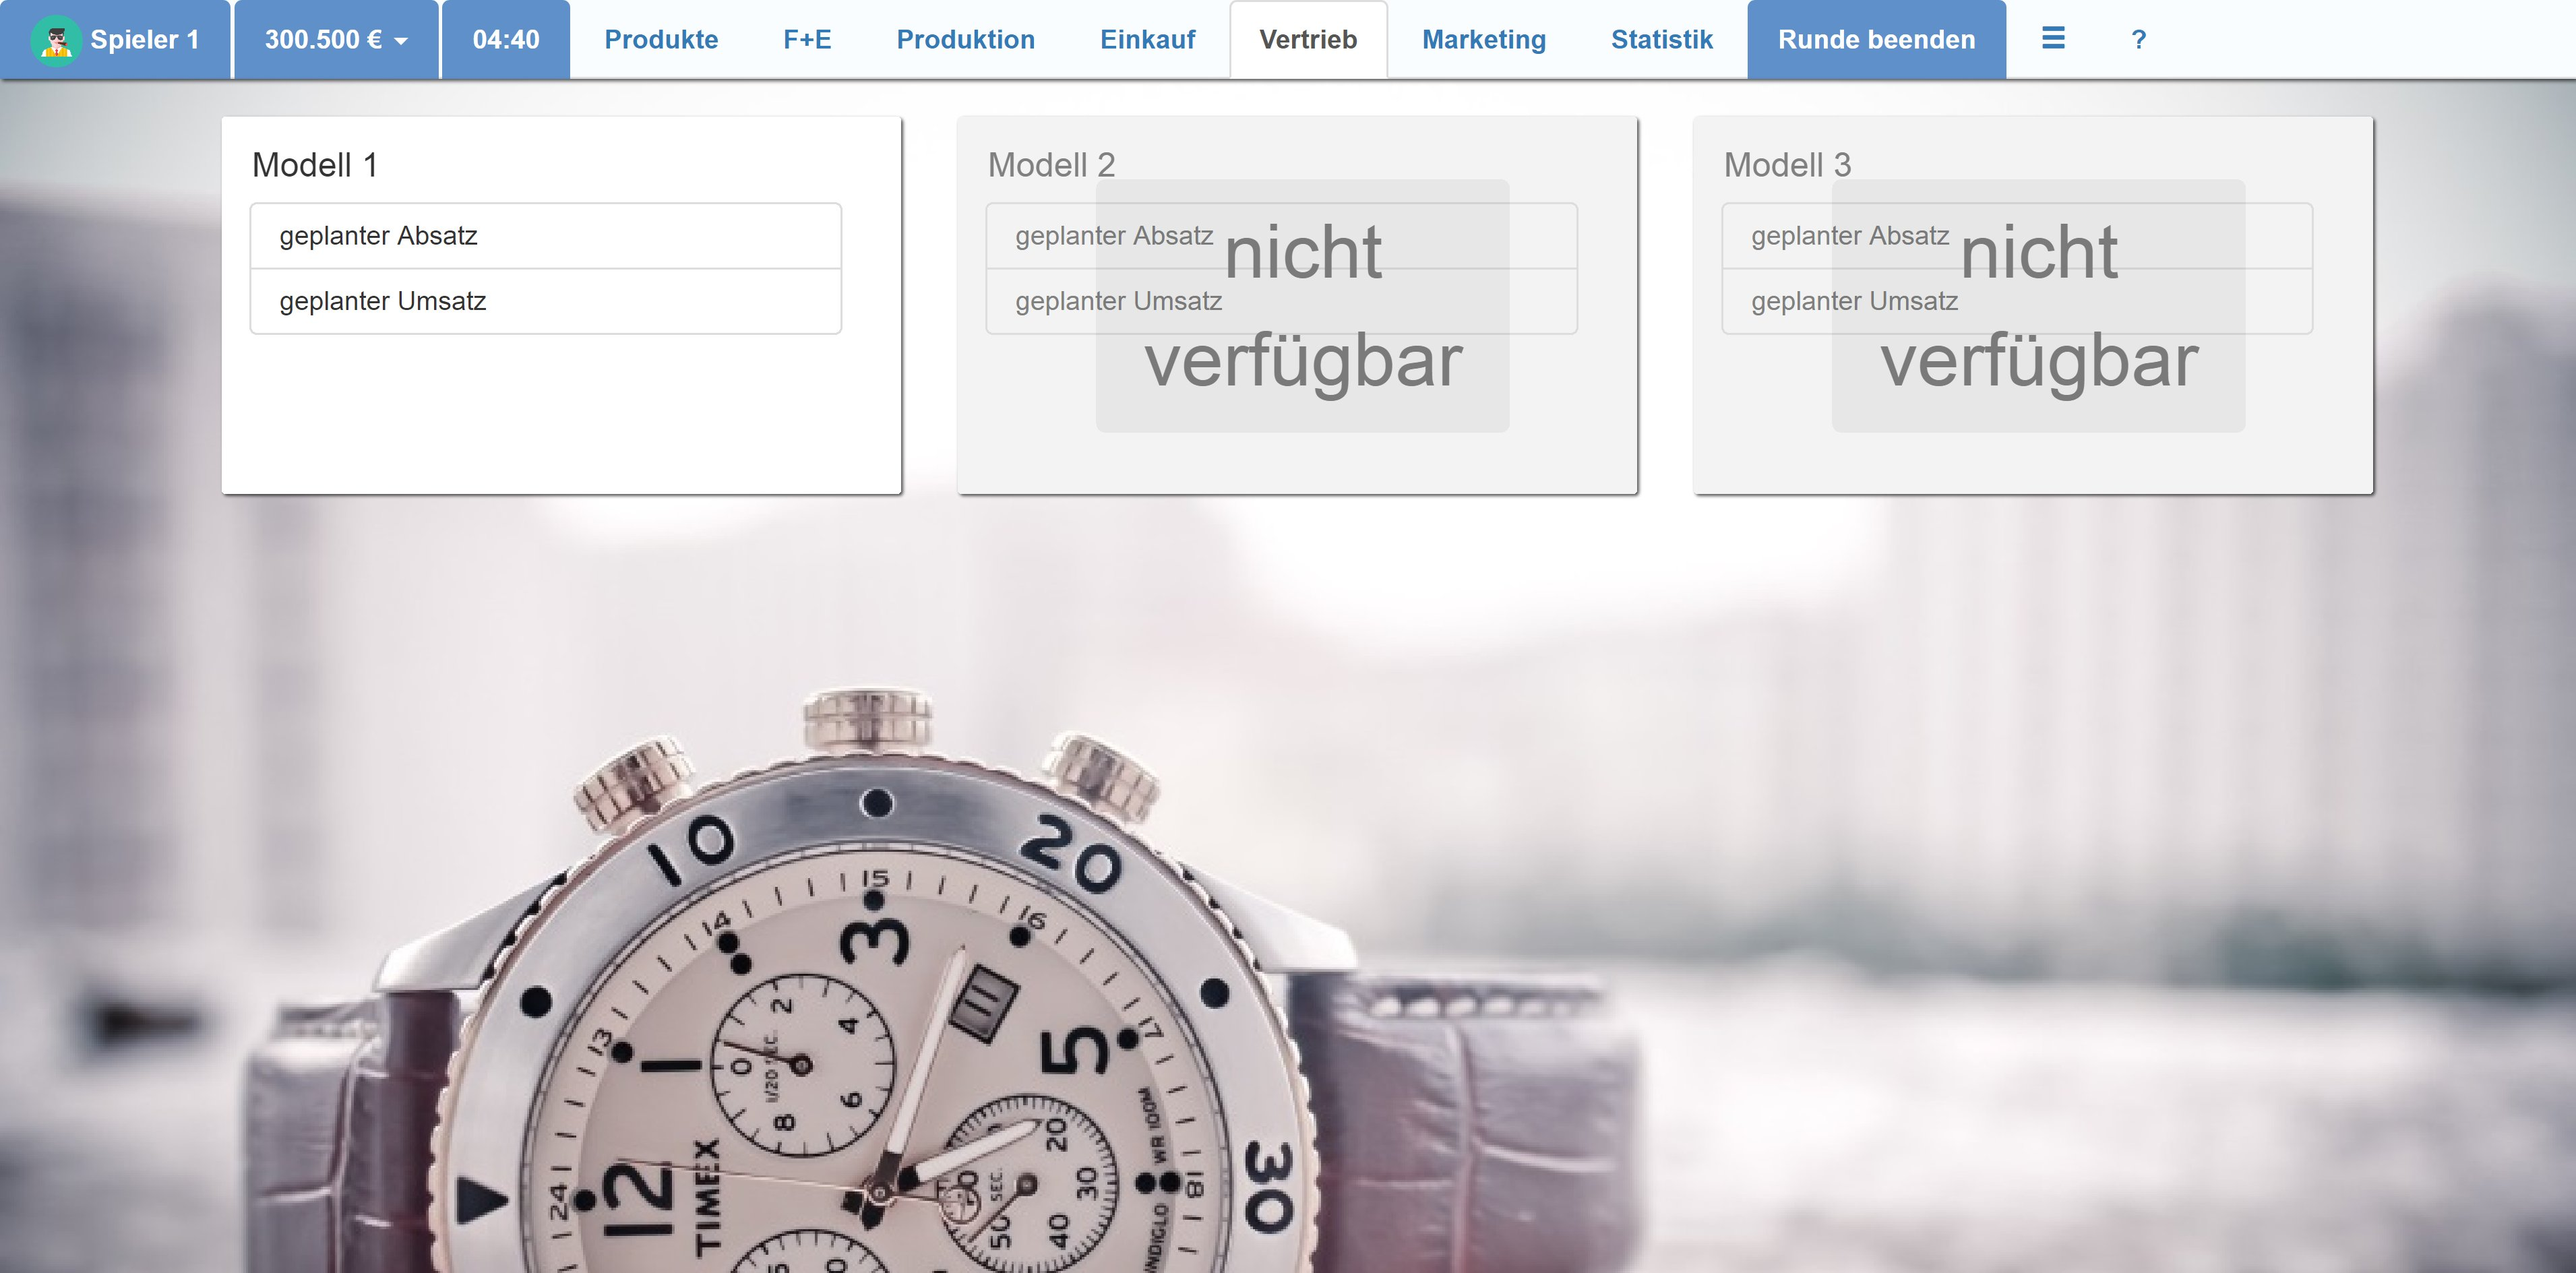
\includegraphics[scale=0.1]{img/bilder_layout/MockUp7.jpg} 
\end{figure}
\begin{figure} 
	\centering
	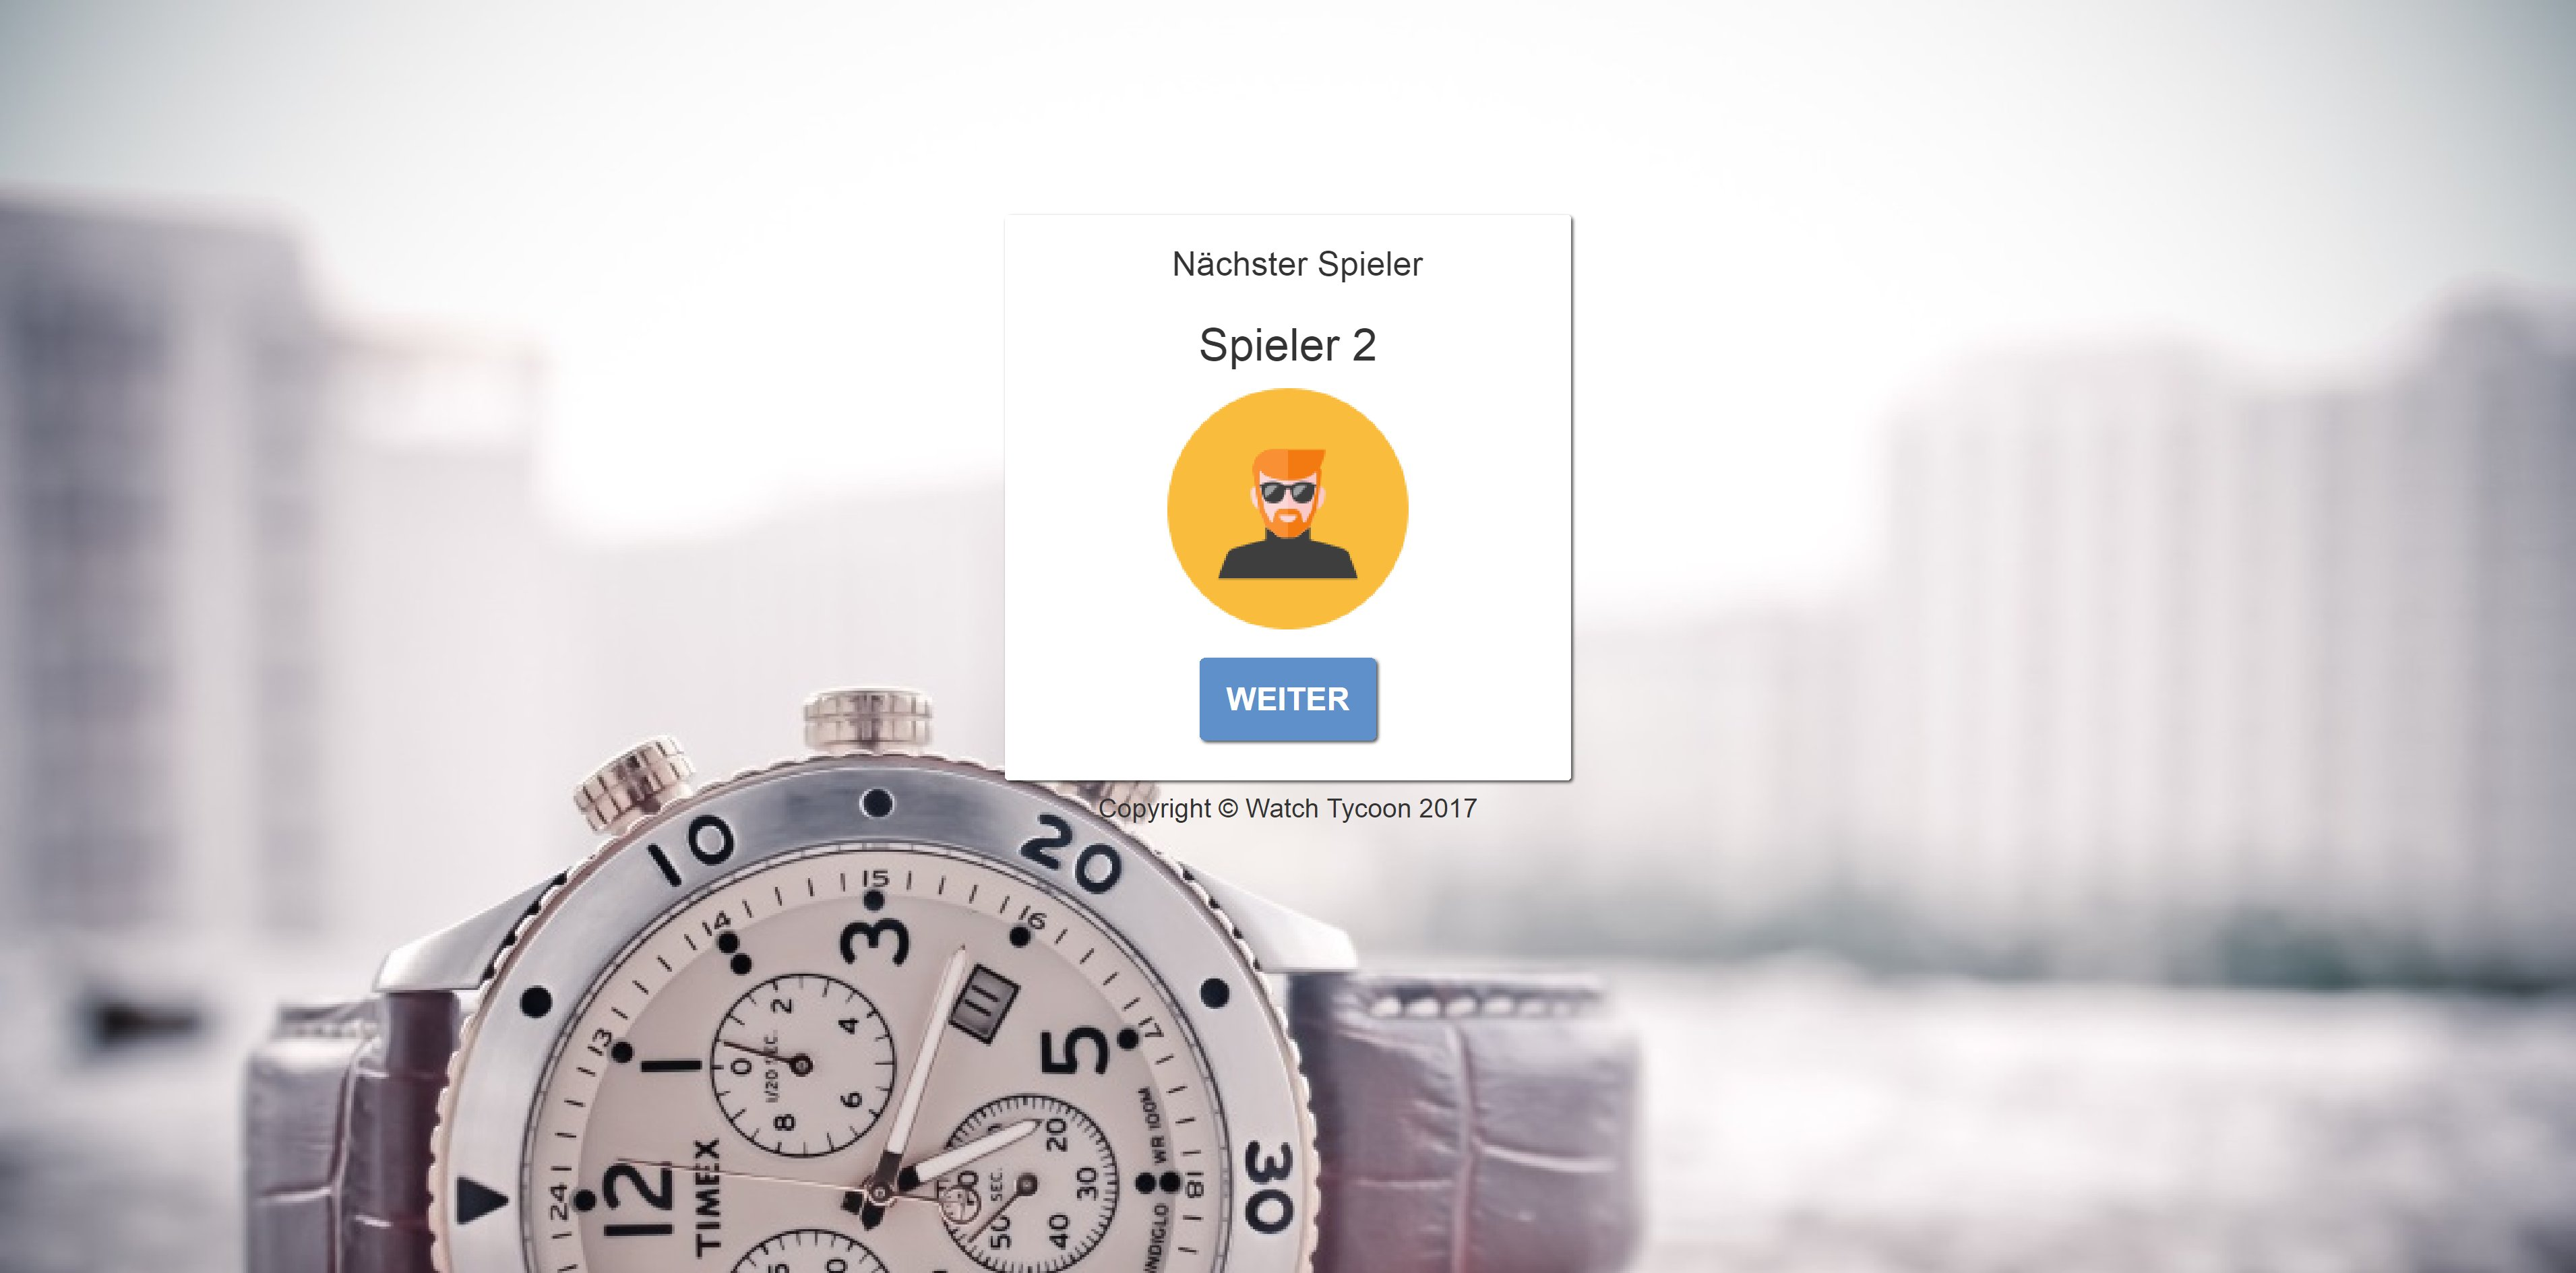
\includegraphics[scale=0.1]{img/bilder_layout/MockUp8.jpg} 
\end{figure}
\begin{figure} 
	\centering
	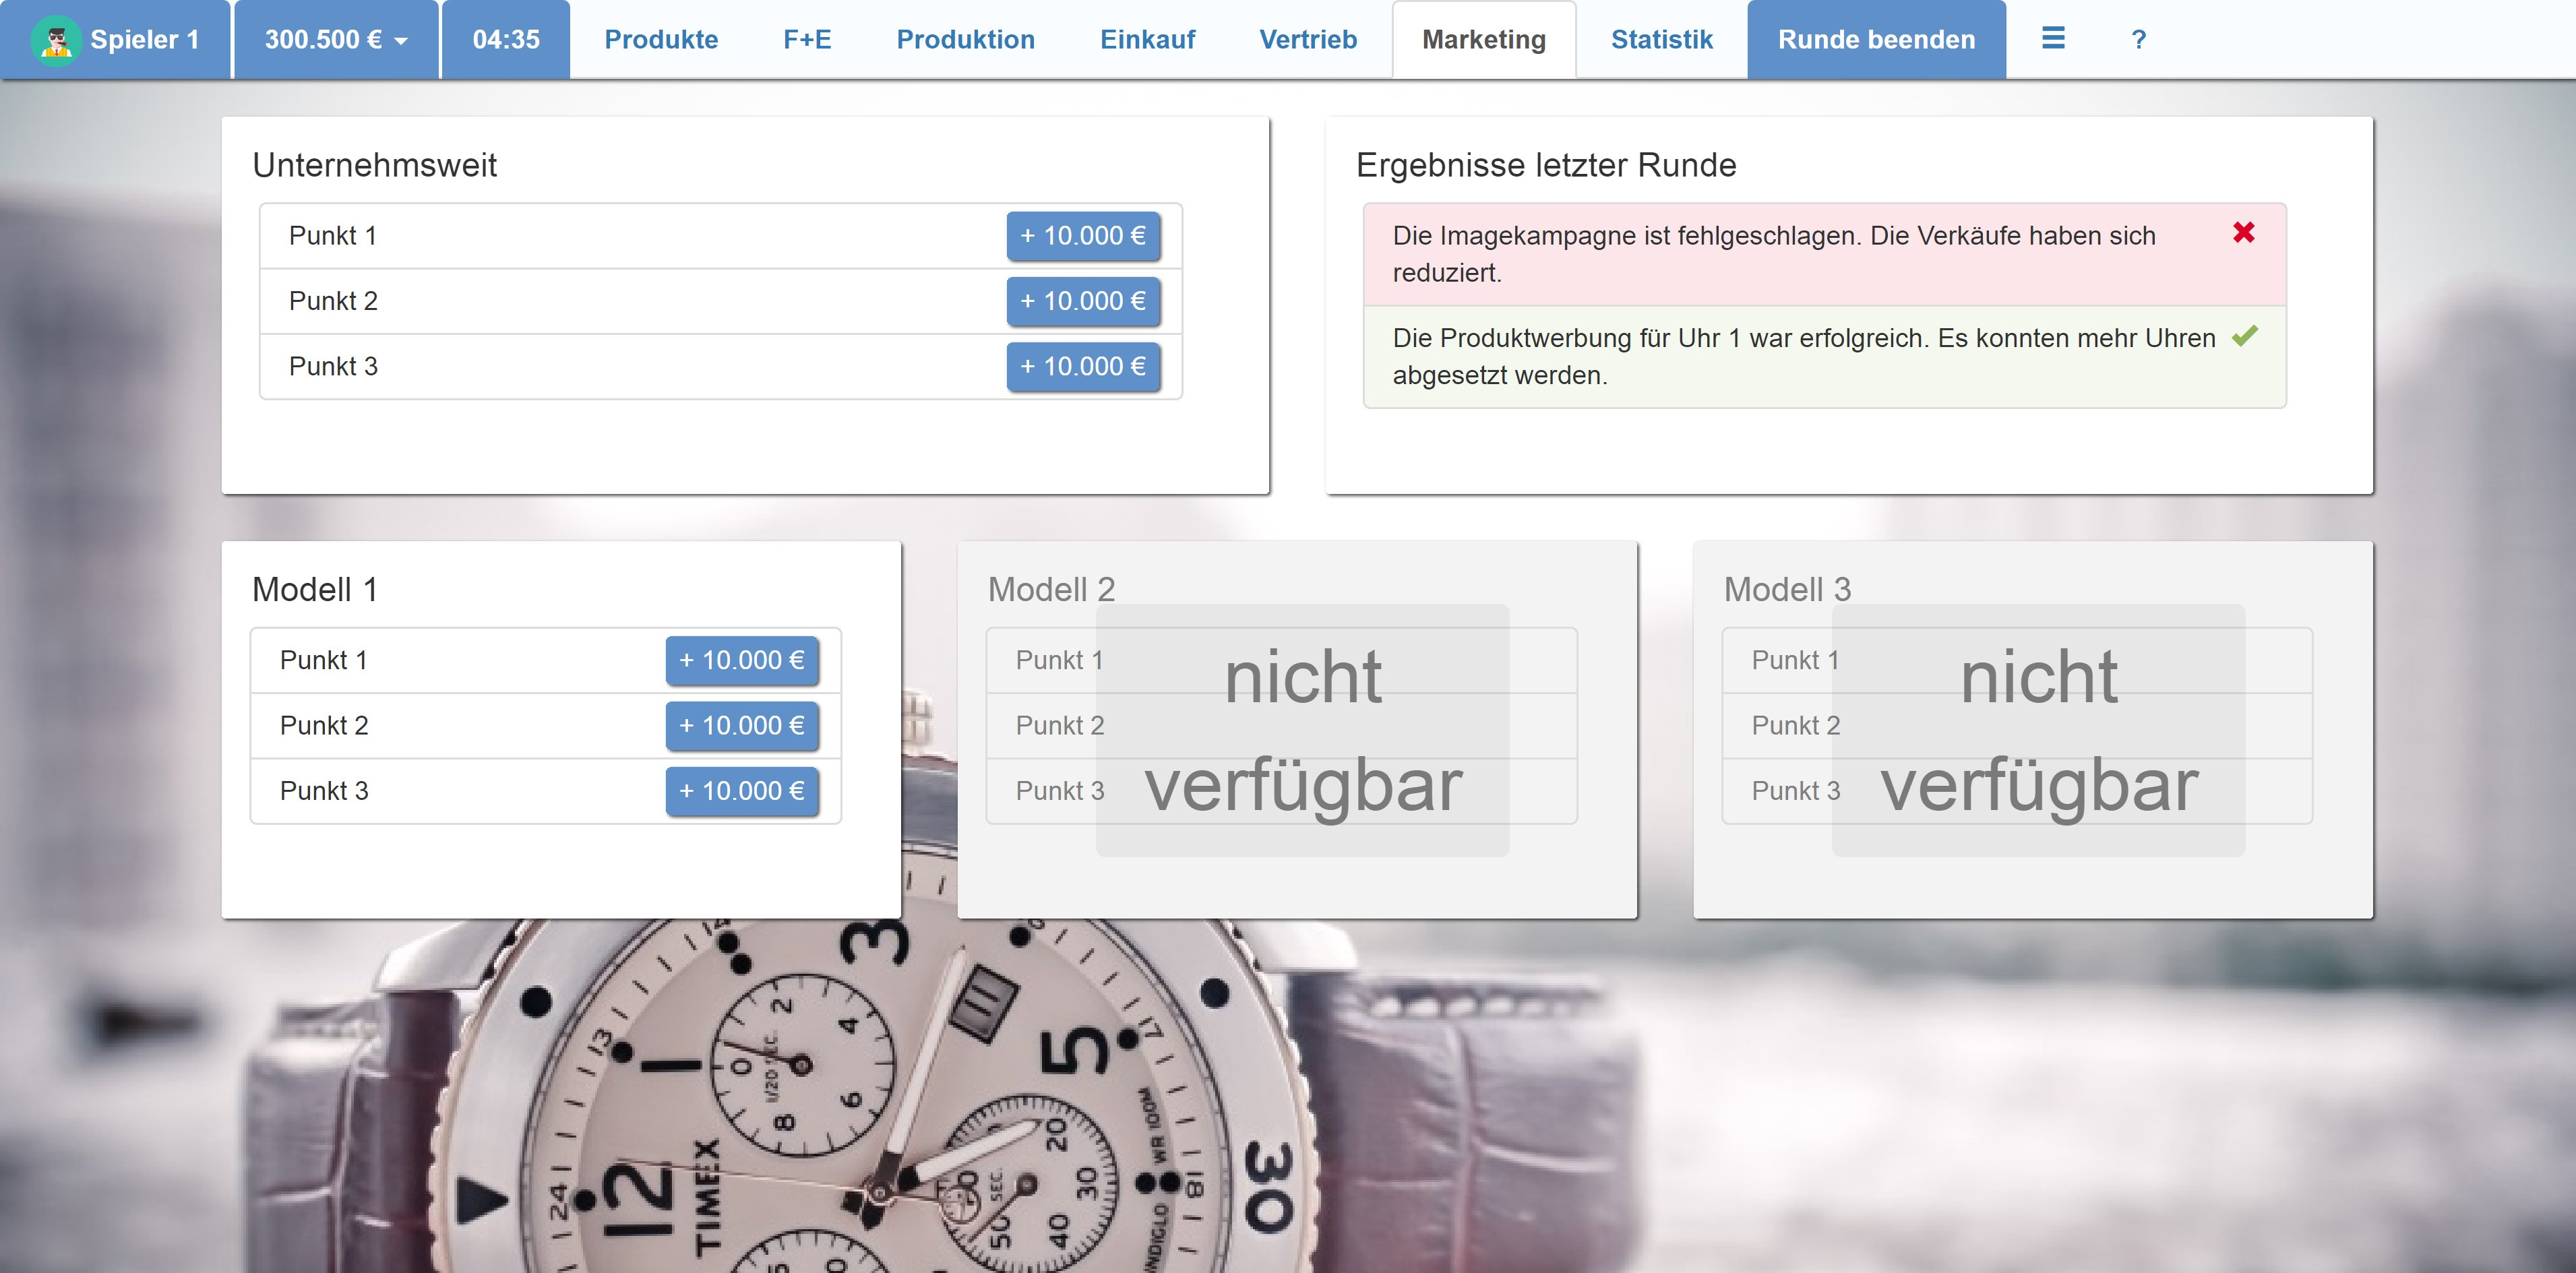
\includegraphics[scale=0.1]{img/bilder_layout/MockUp9.jpg} 
\end{figure}
\clearpage
\subsection{Finales UI}
\begin{figure} [h]
	\centering
	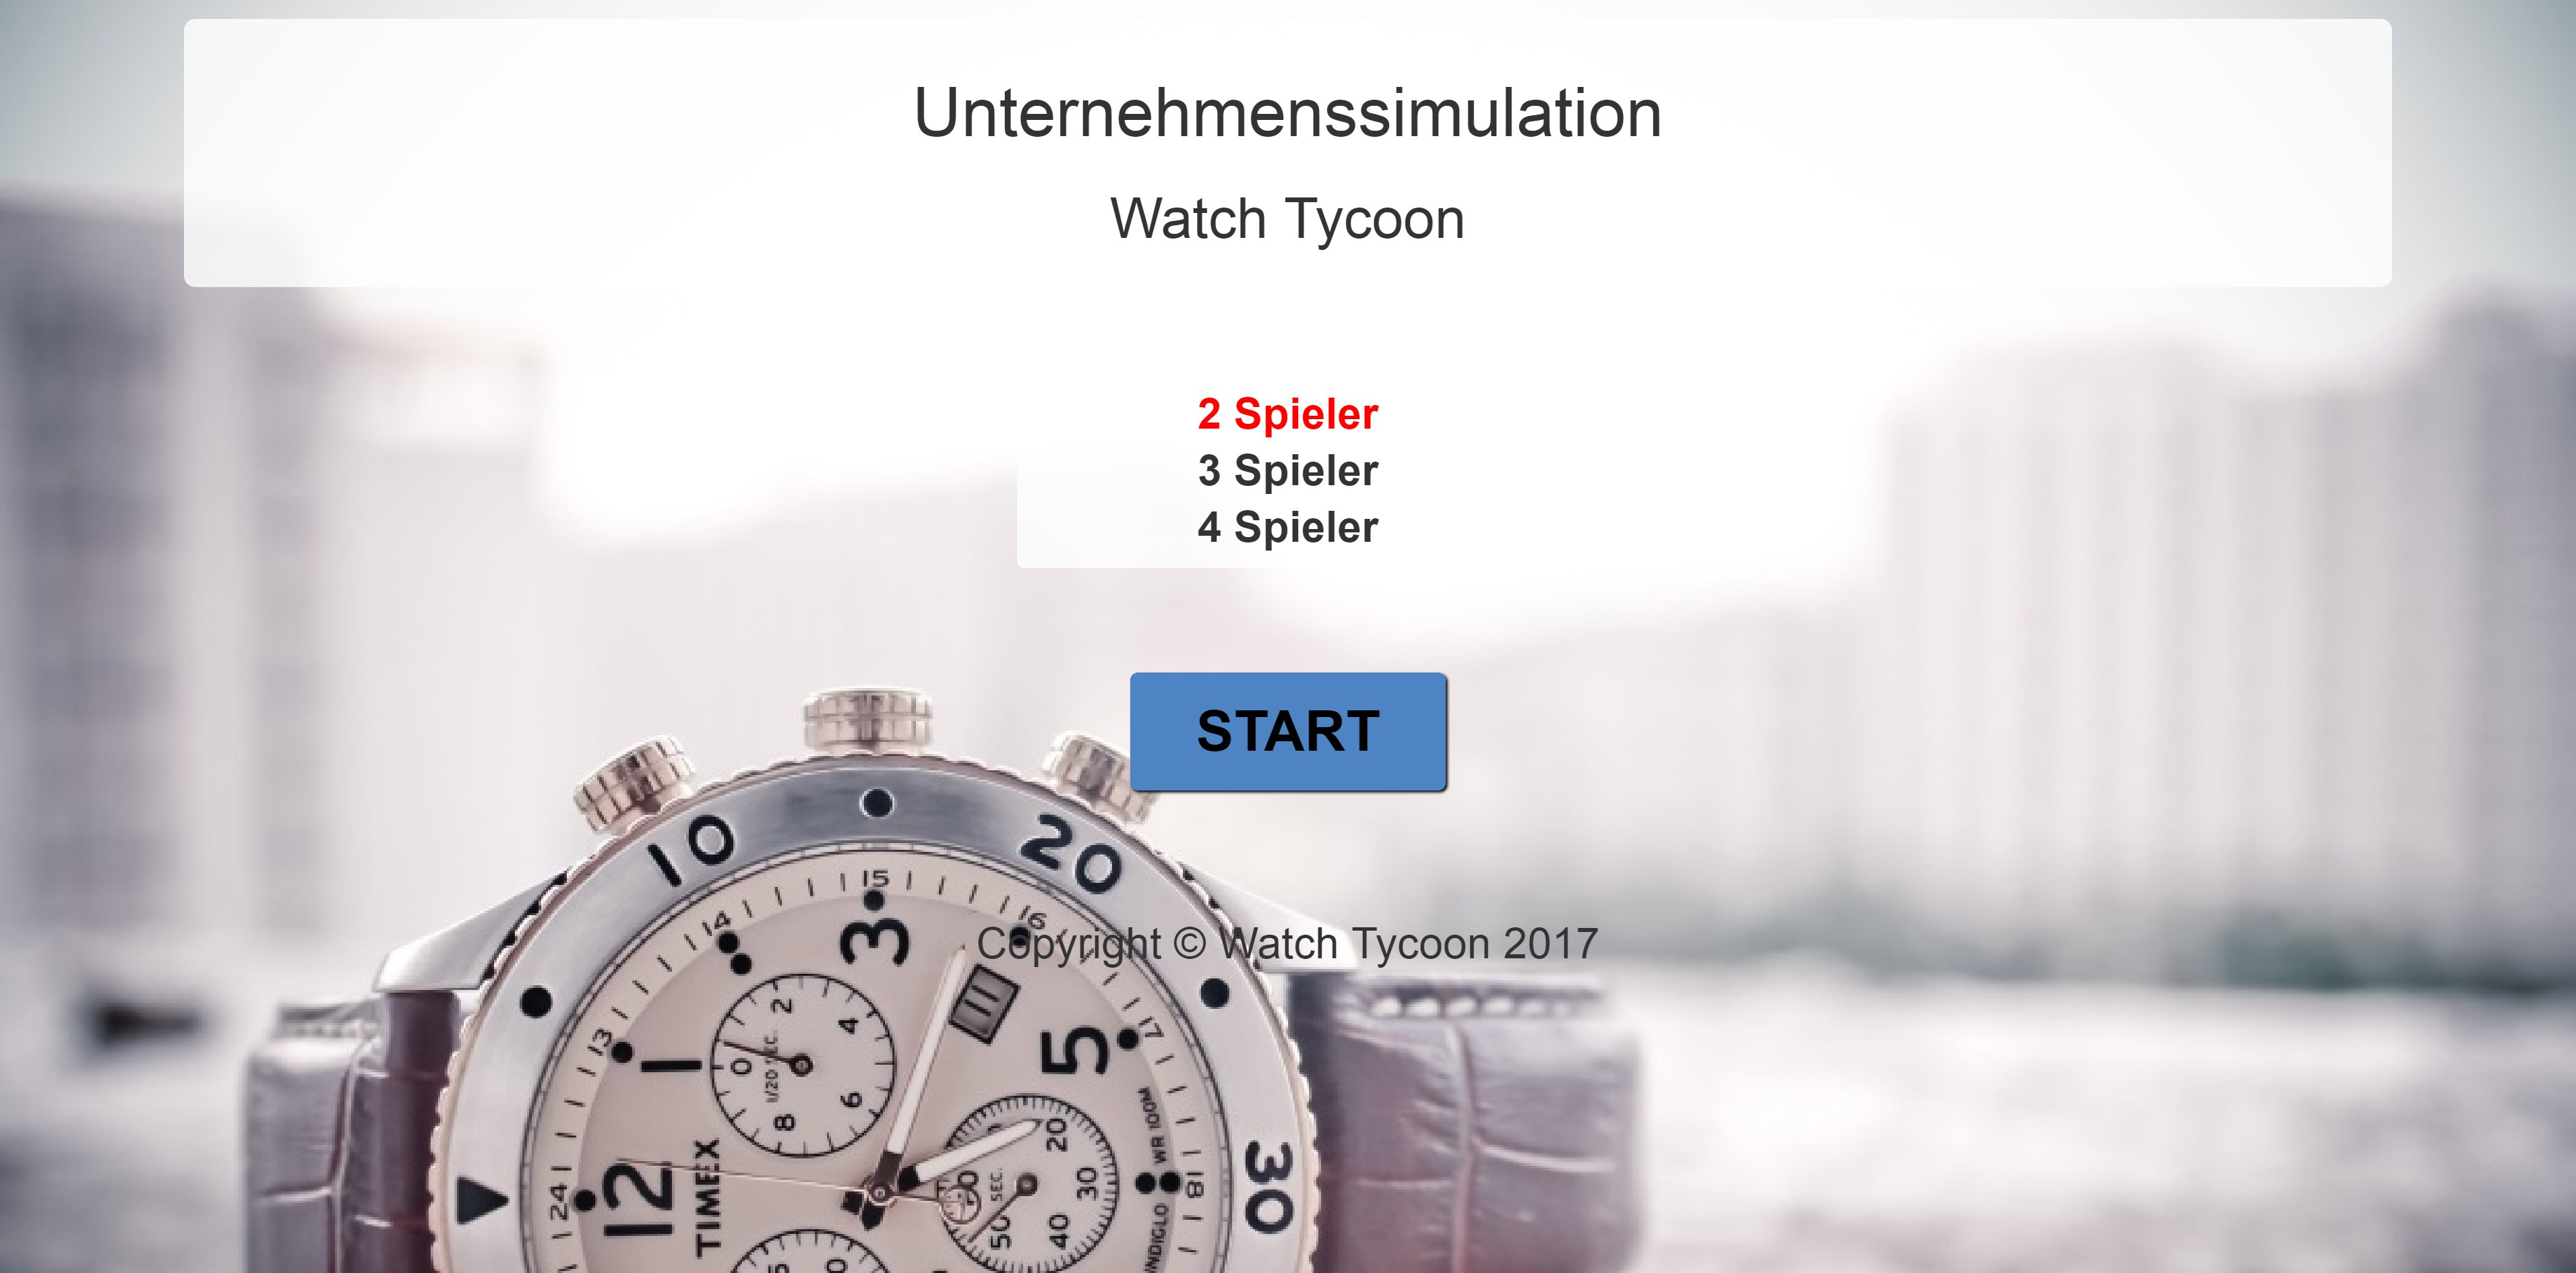
\includegraphics[scale=0.1]{img/bilder_layout/Spiel1.jpg} 
\end{figure}
\begin{figure} [h]
	\centering
	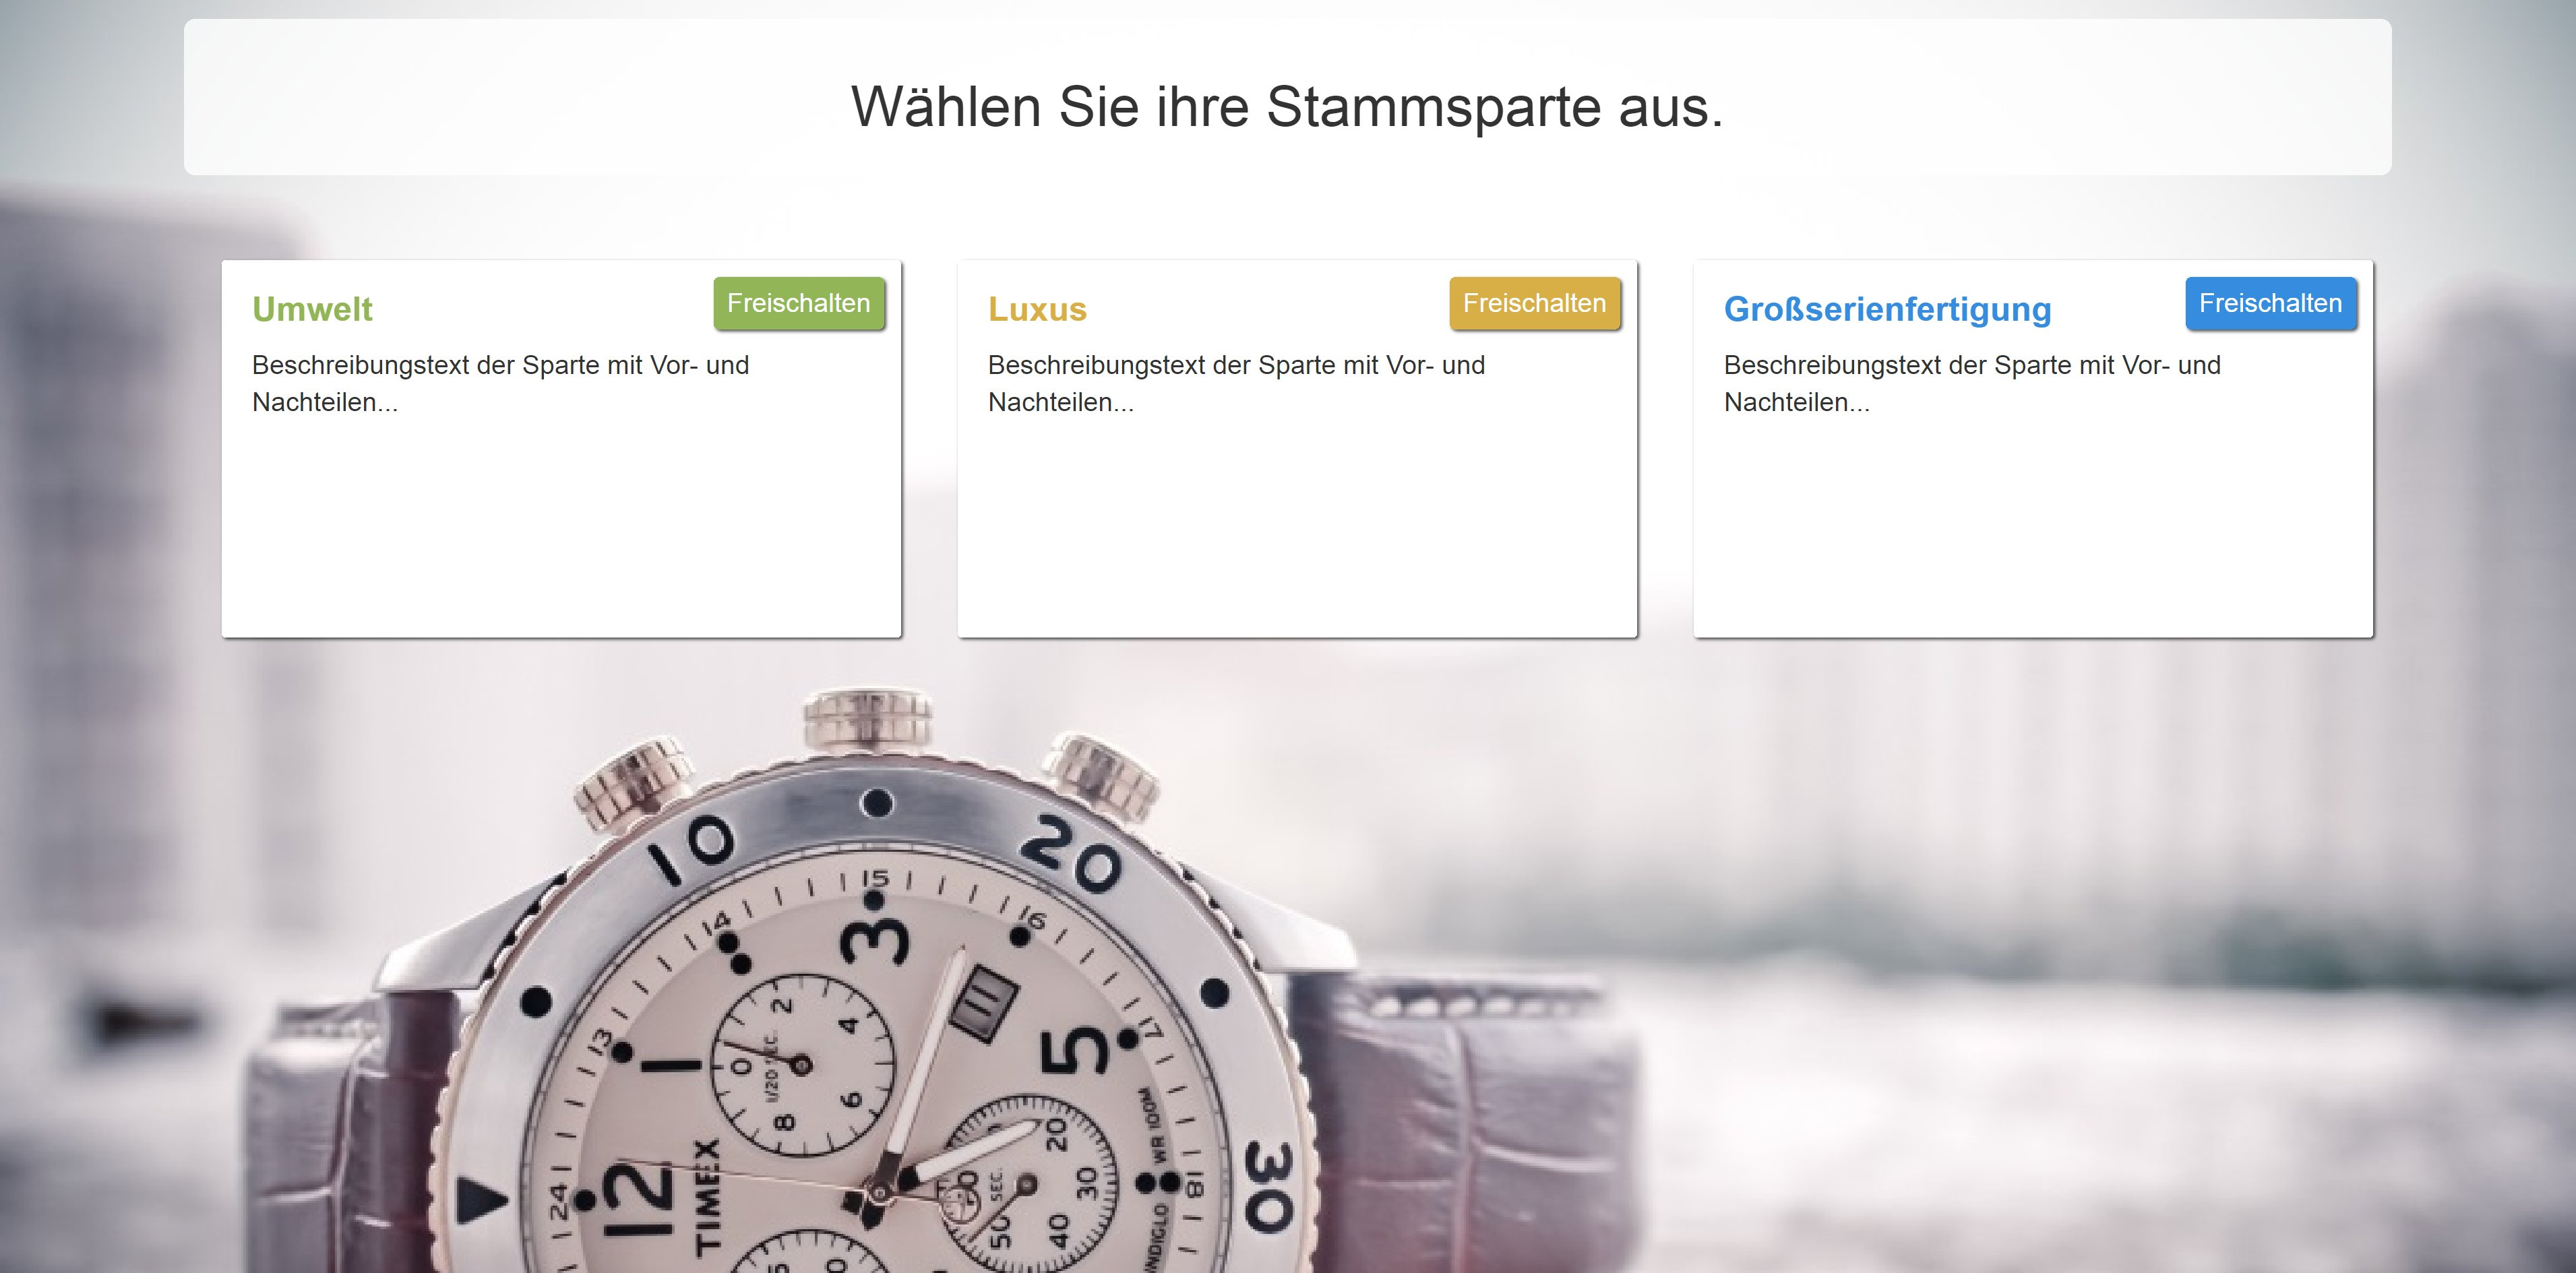
\includegraphics[scale=0.1]{img/bilder_layout/Spiel2.jpg} 
\end{figure}
\begin{figure} 
	\centering
	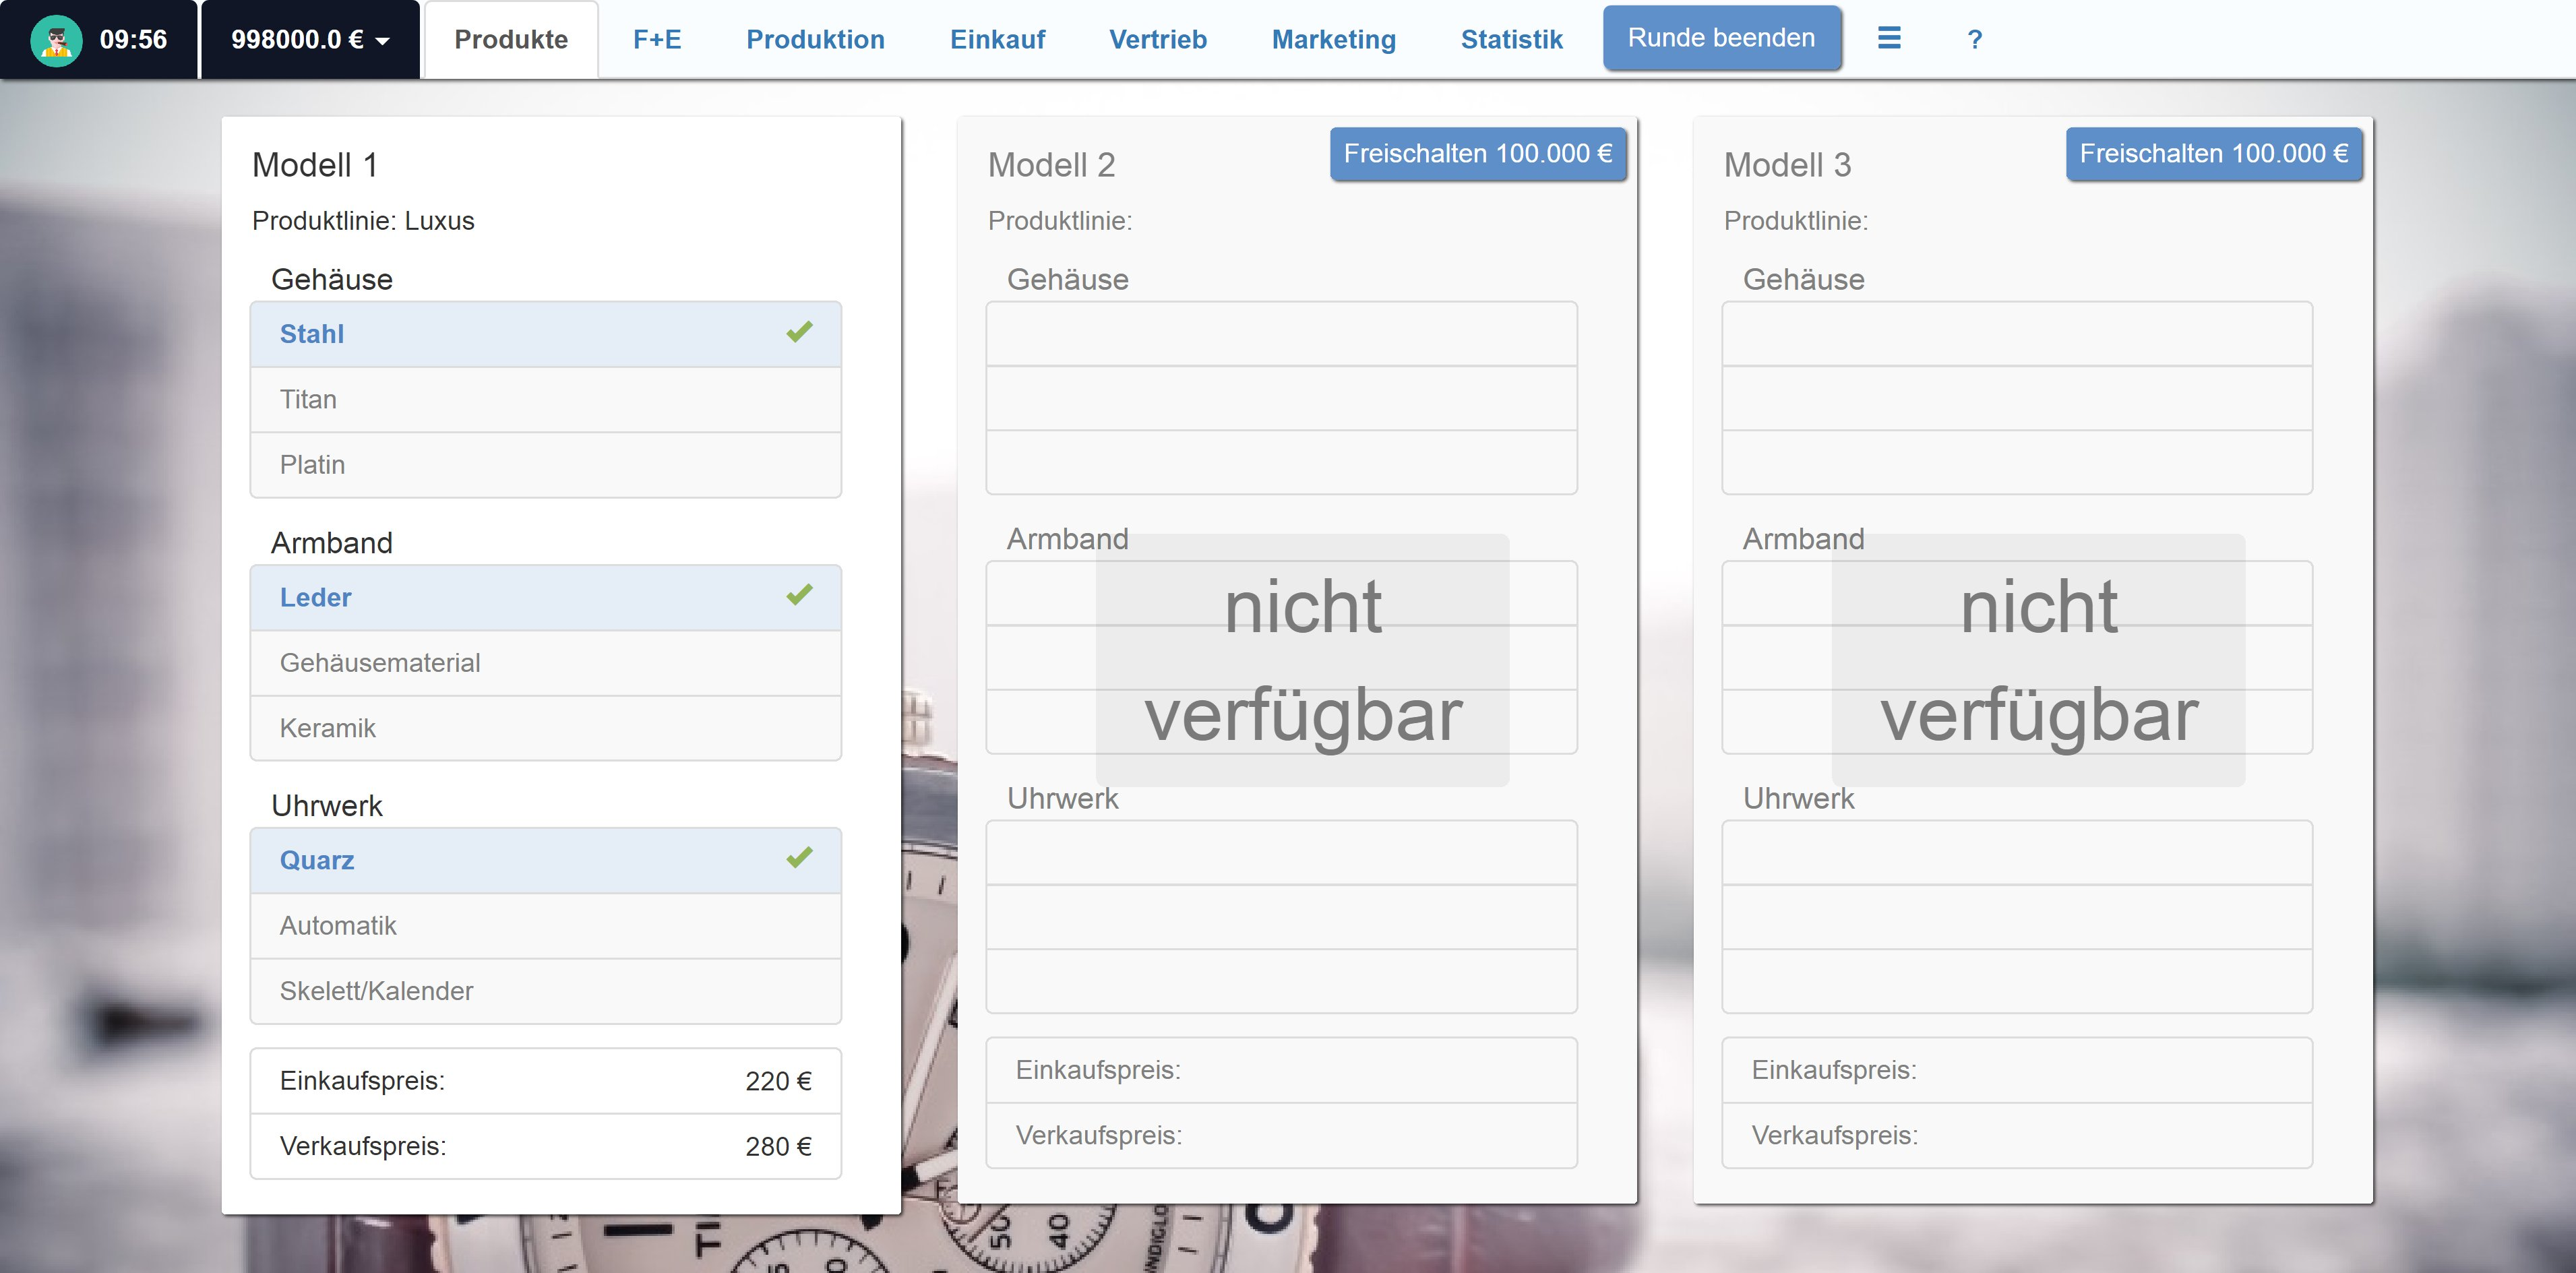
\includegraphics[scale=0.1]{img/bilder_layout/Spiel3.jpg} 
\end{figure}
\begin{figure} 
	\centering
	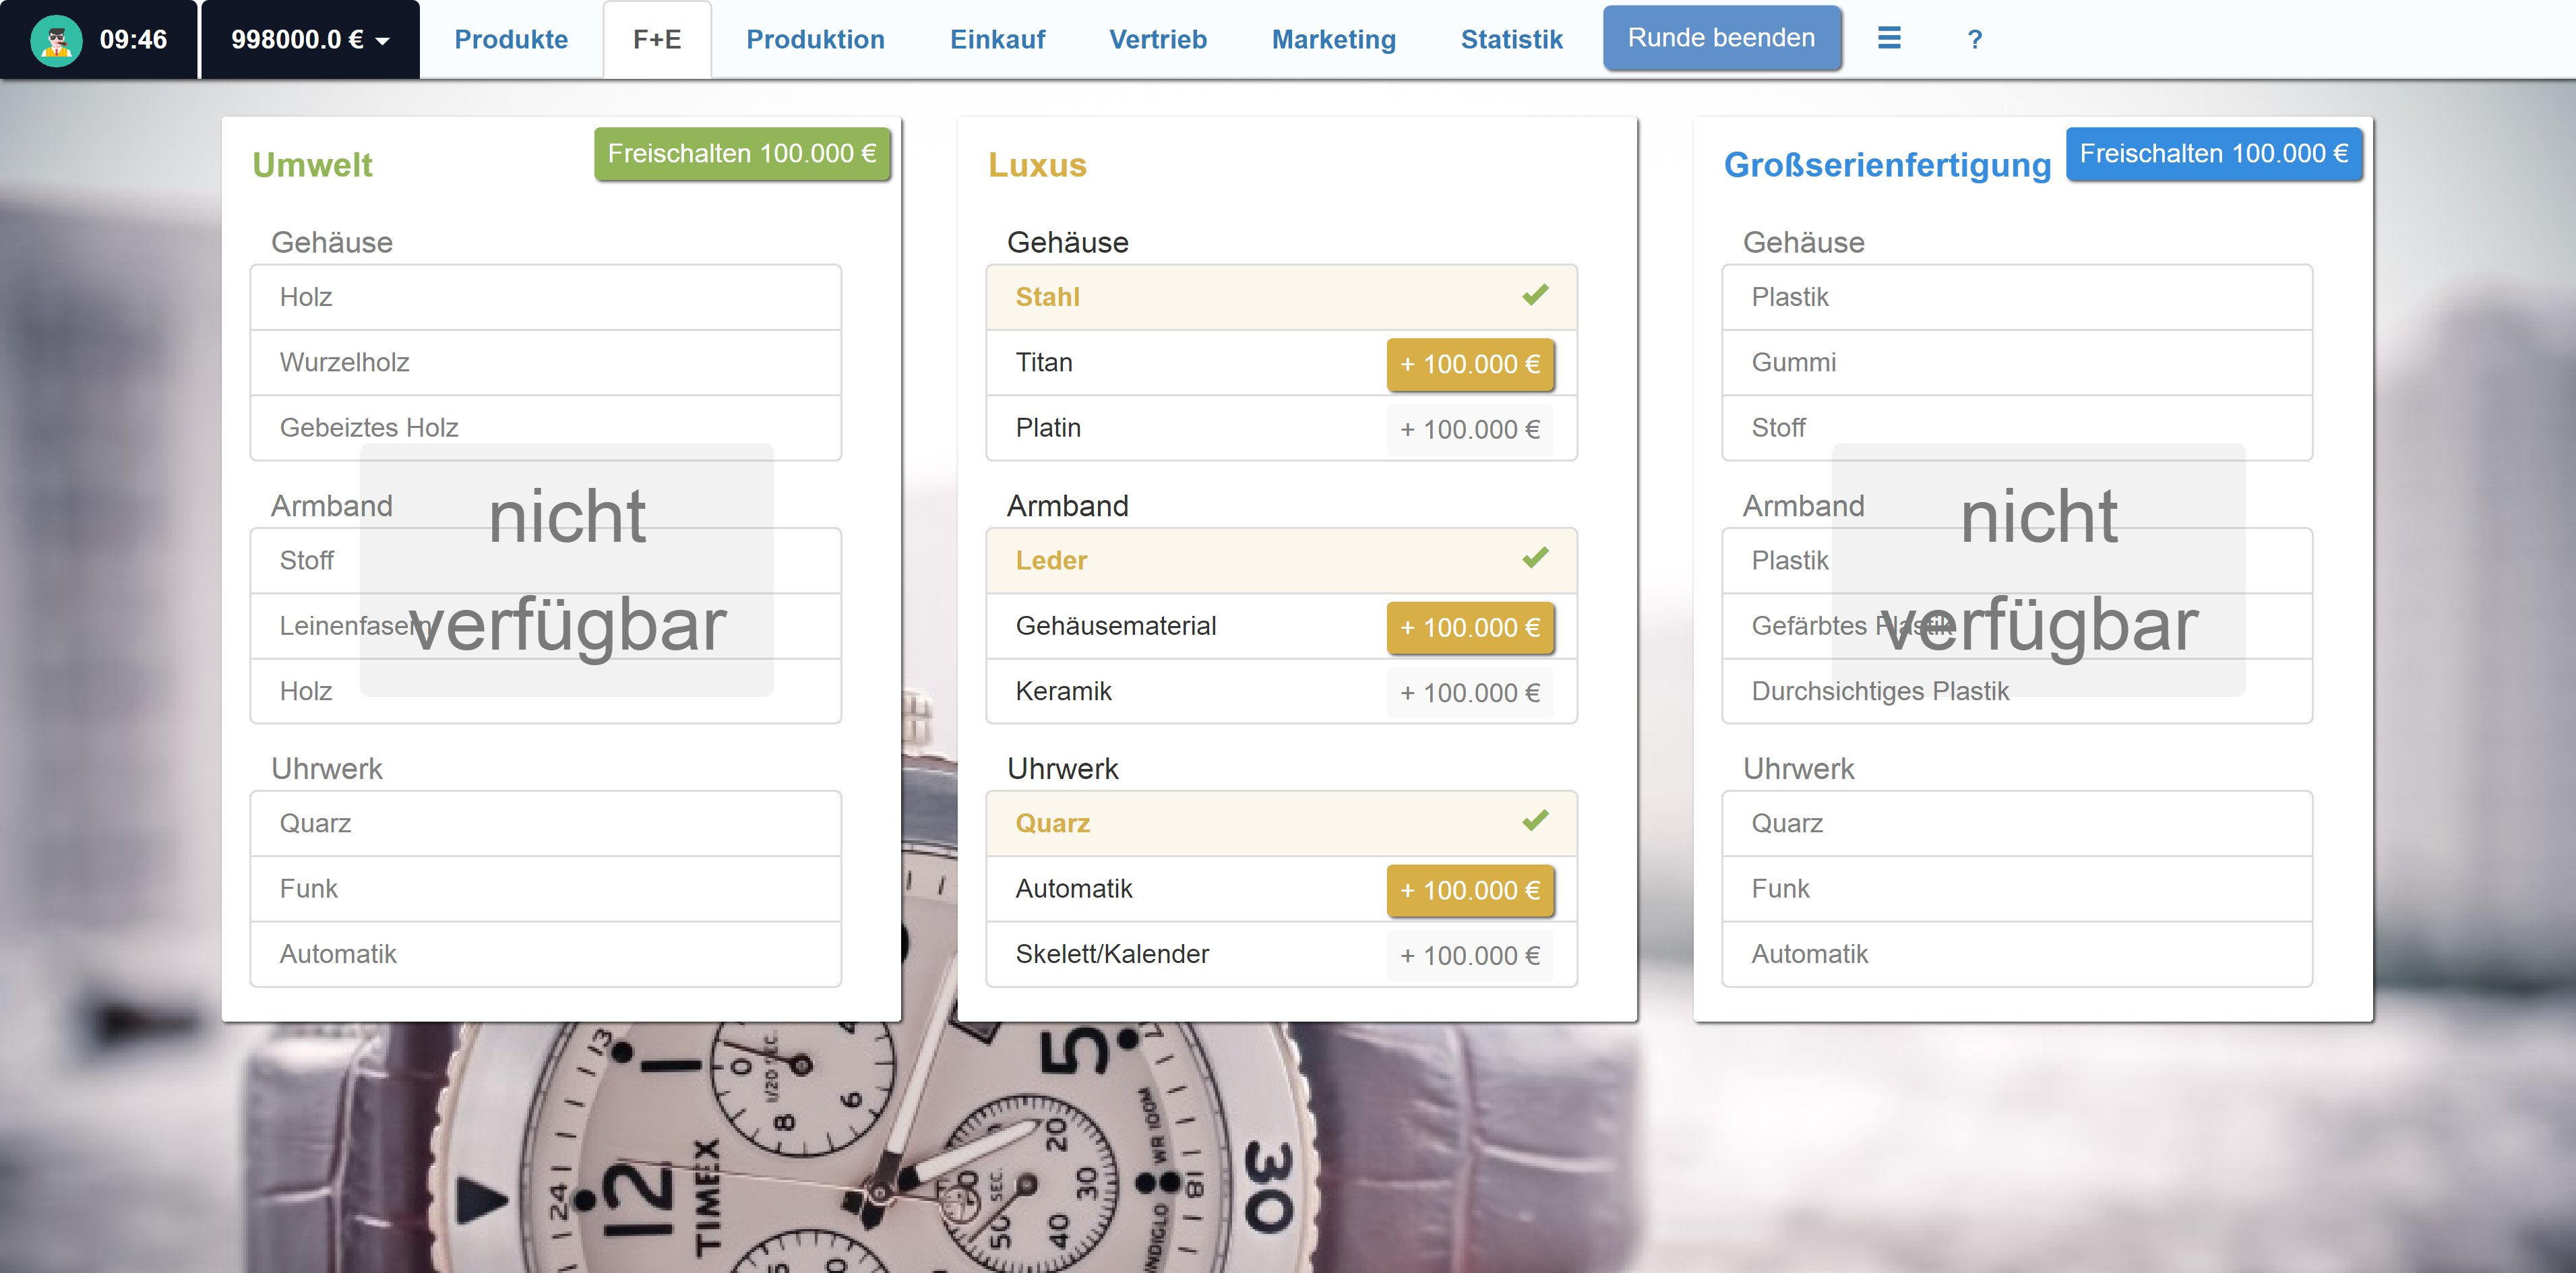
\includegraphics[scale=0.1]{img/bilder_layout/Spiel4.jpg} 
\end{figure}
\begin{figure} 
	\centering
	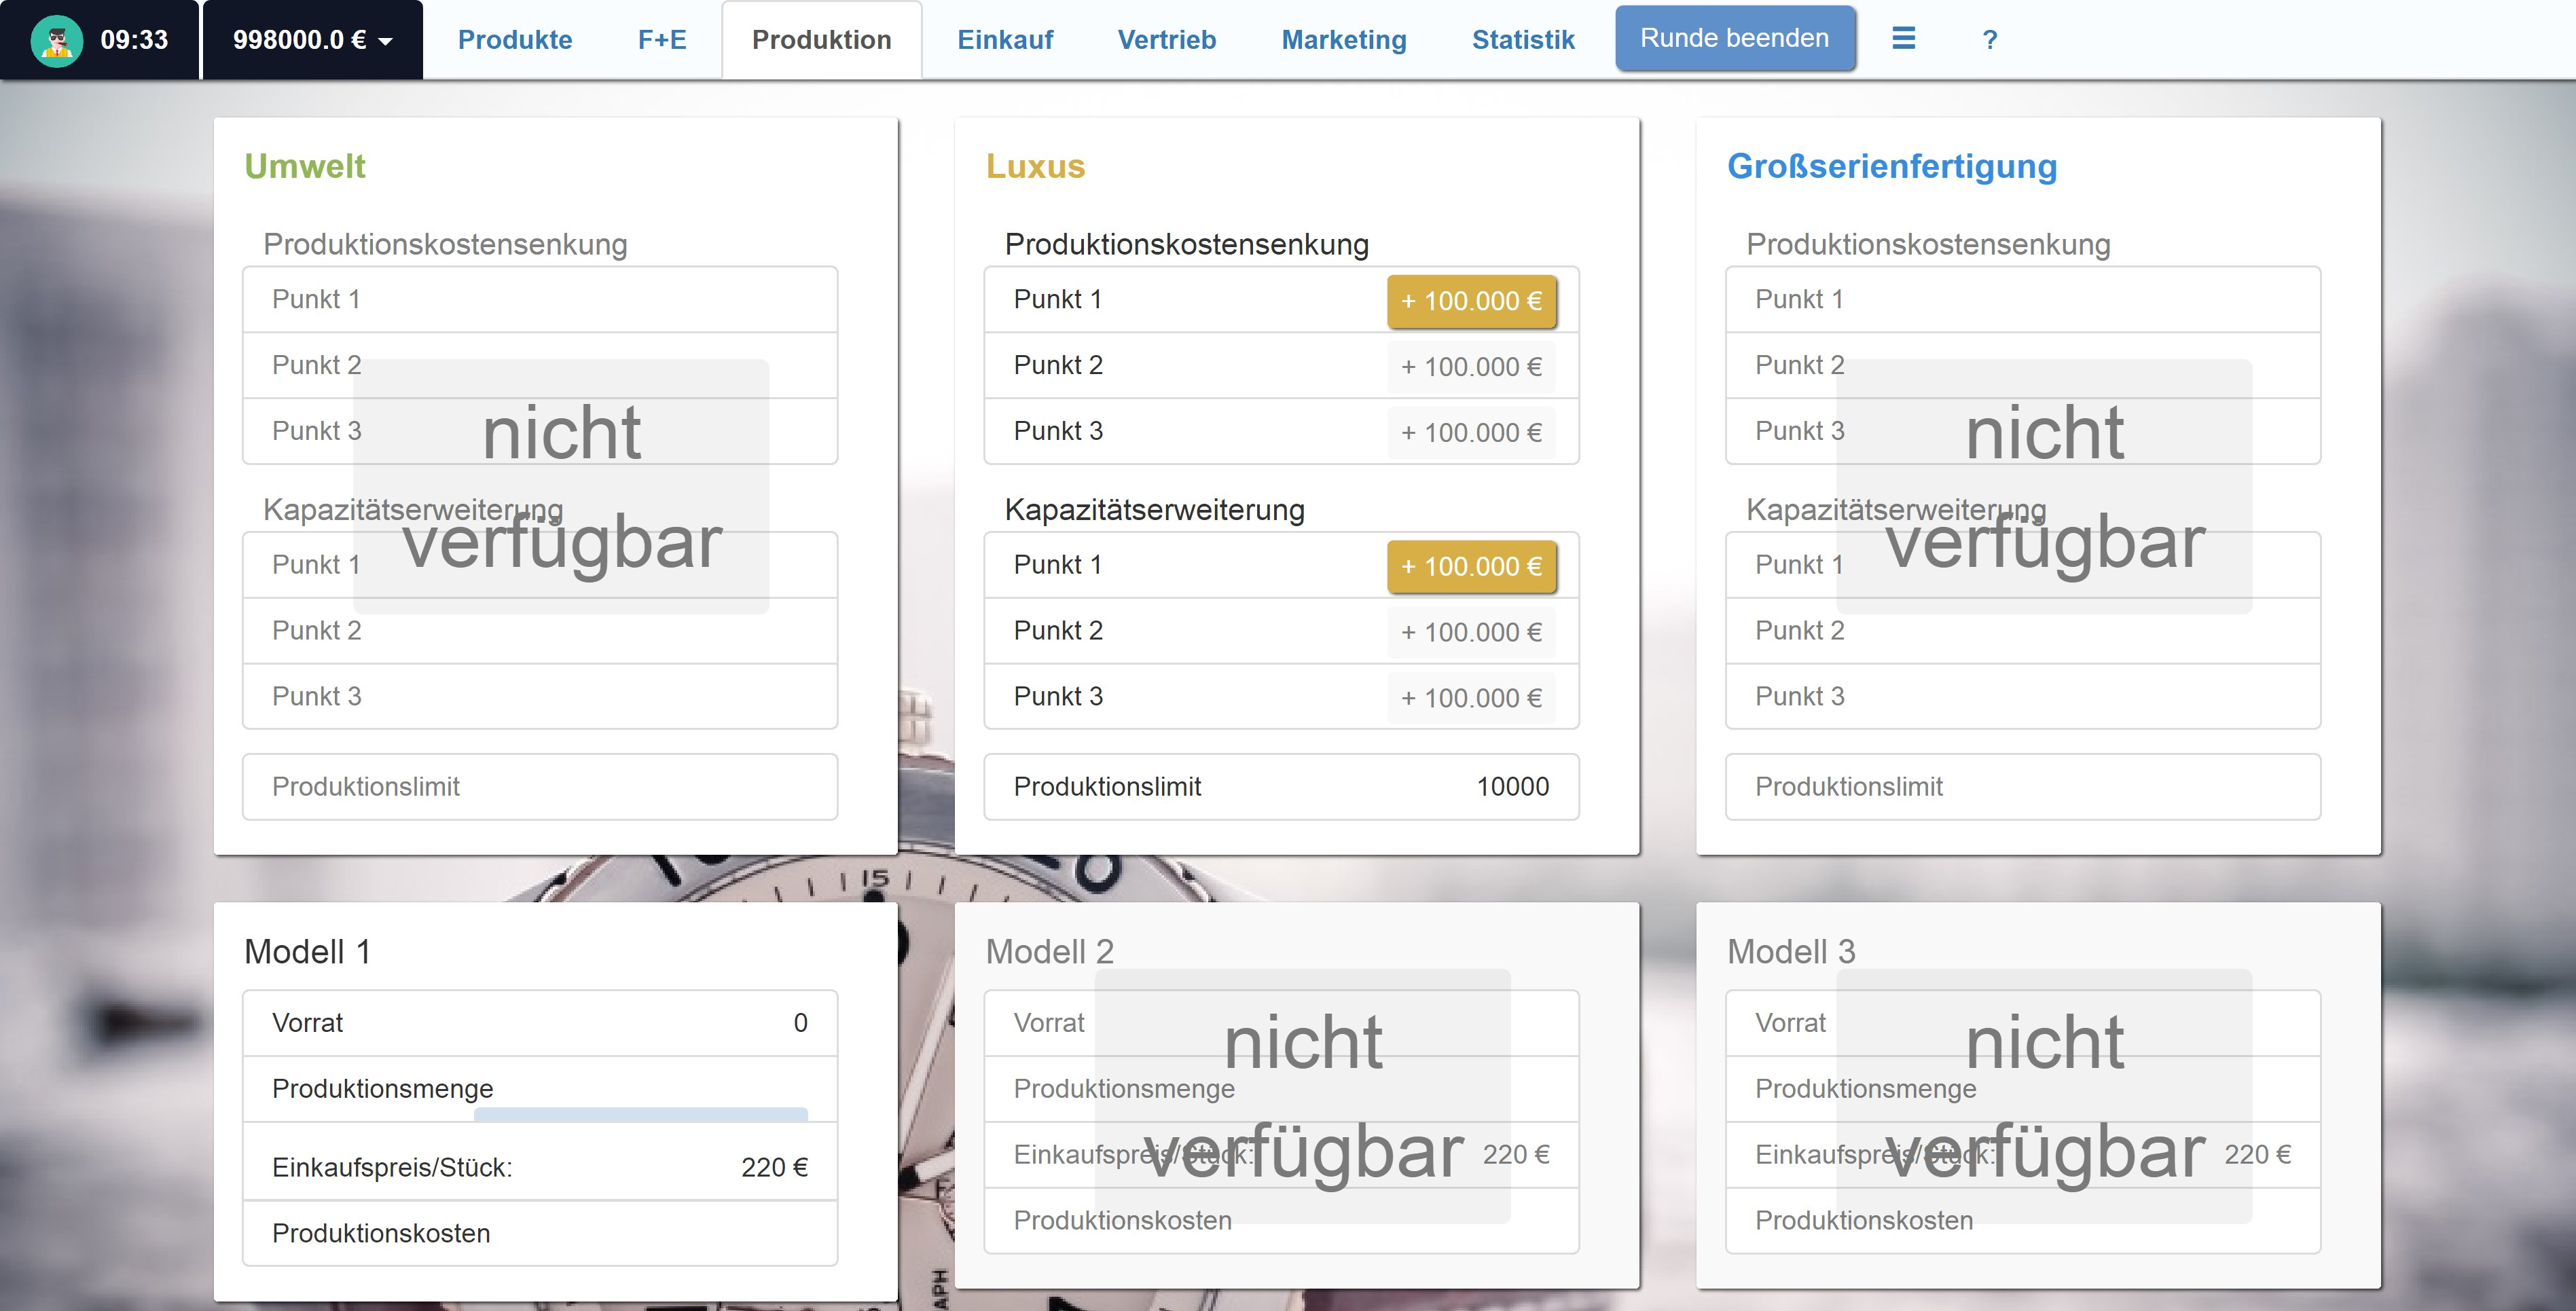
\includegraphics[scale=0.1]{img/bilder_layout/Spiel5.jpg} 
\end{figure}
\begin{figure} 
	\centering
	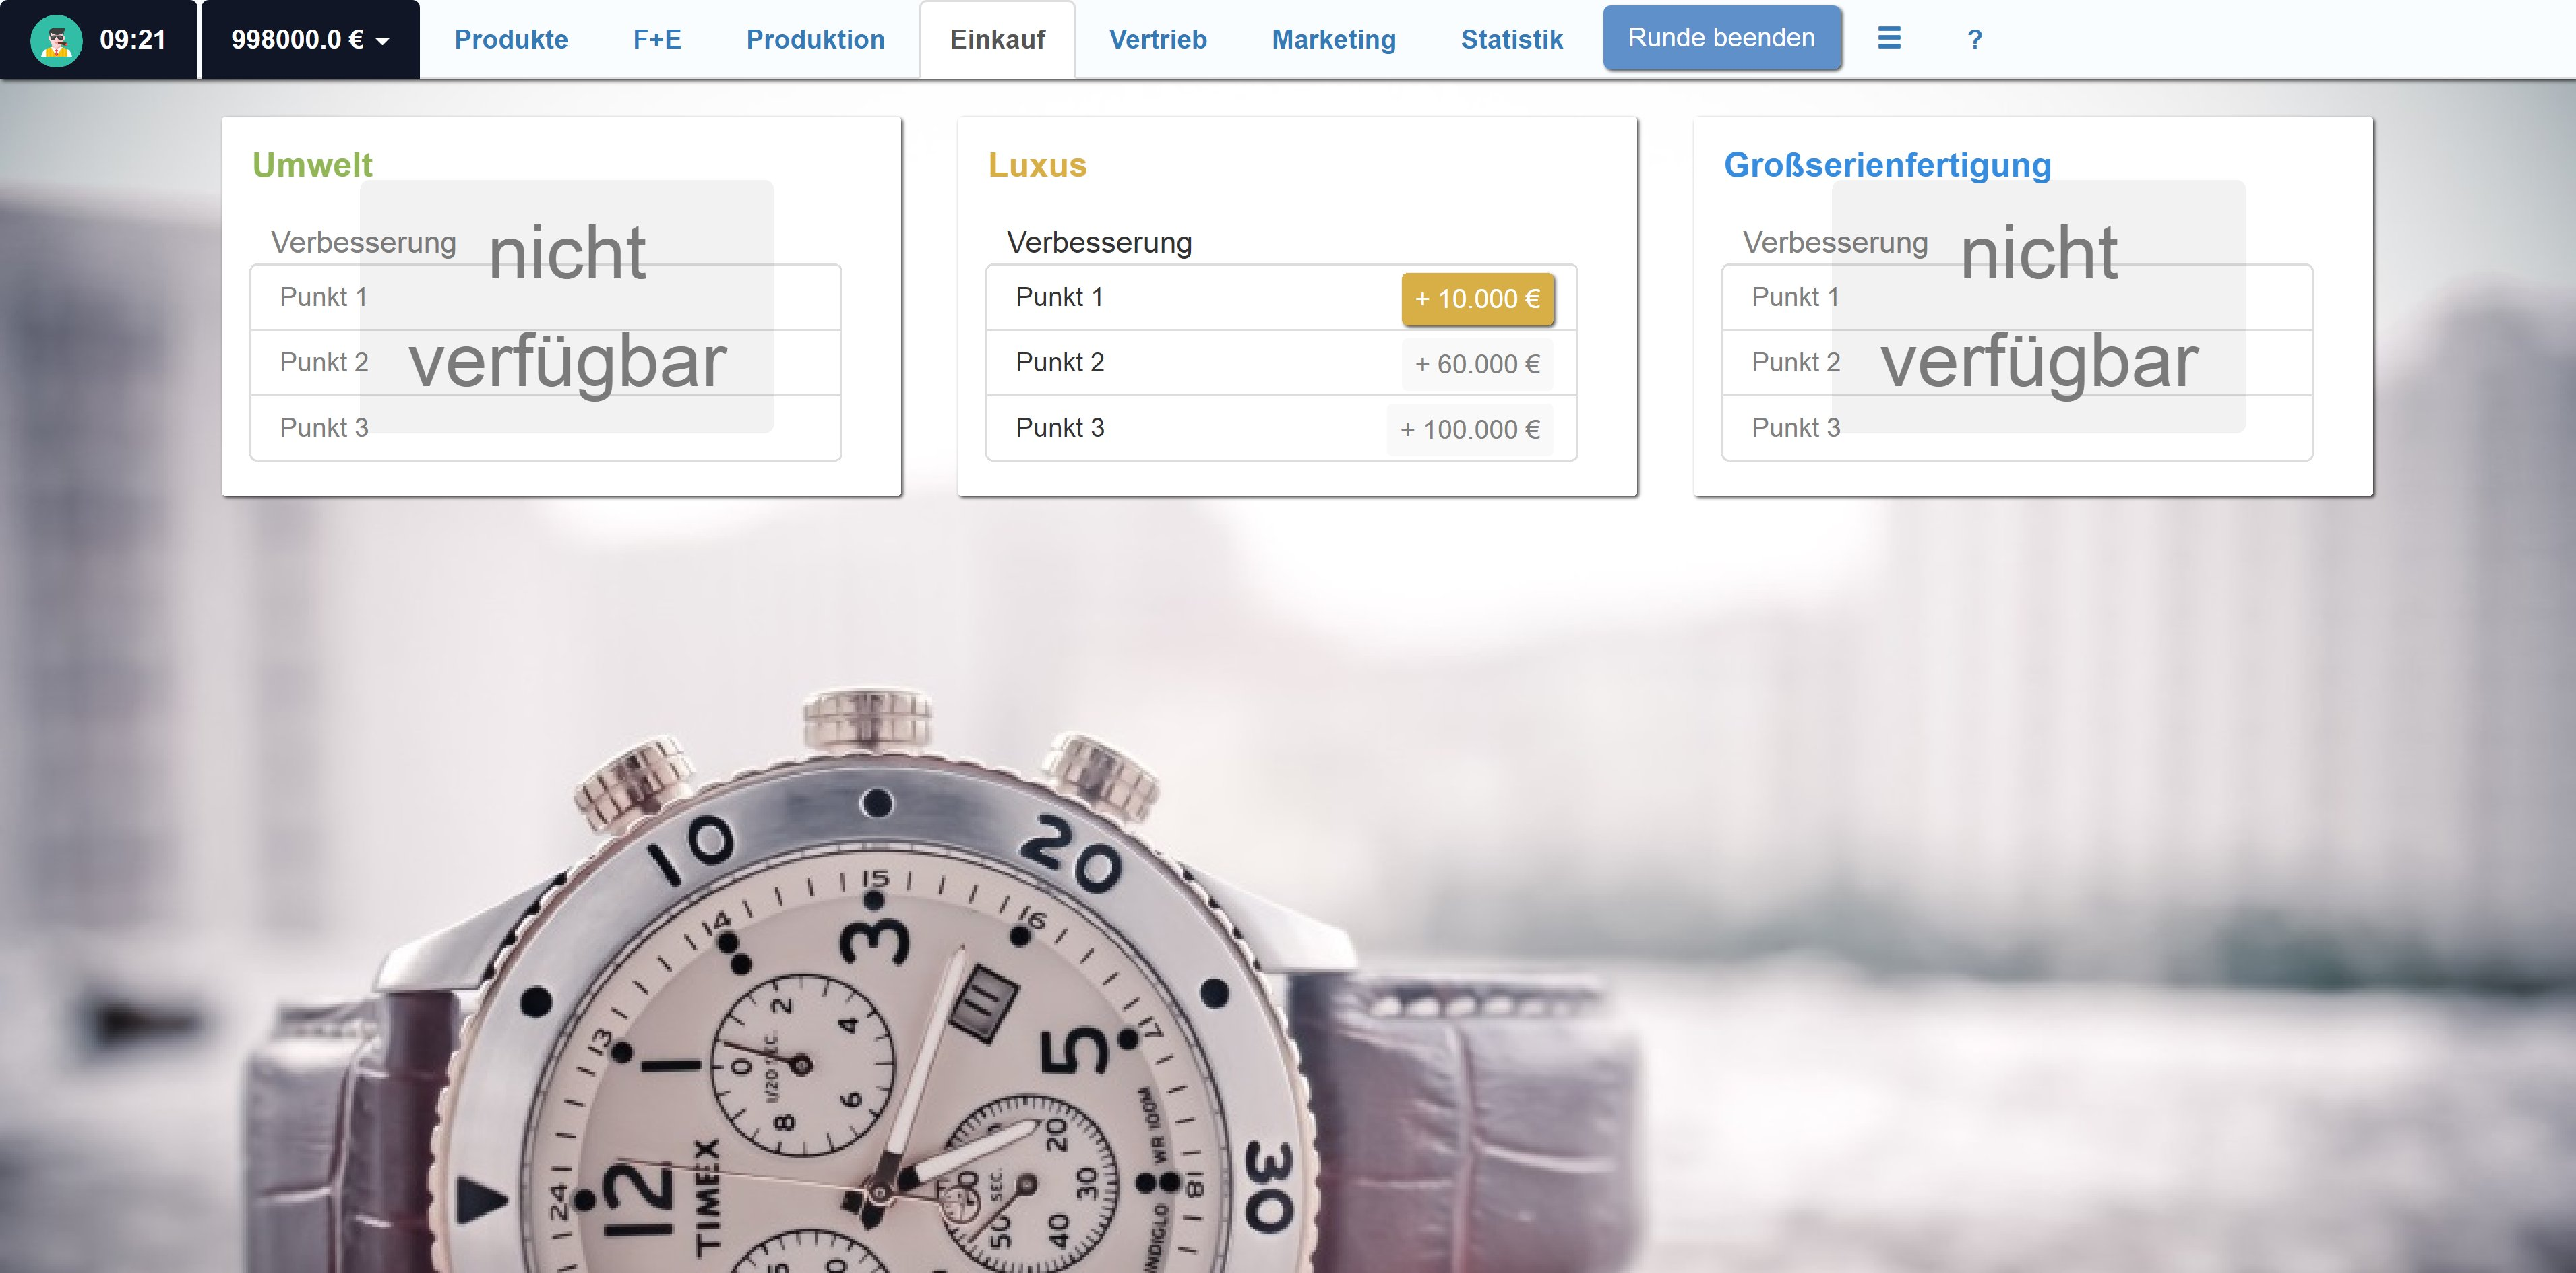
\includegraphics[scale=0.1]{img/bilder_layout/Spiel6.jpg} 
\end{figure}
\begin{figure} [h]
	\centering
	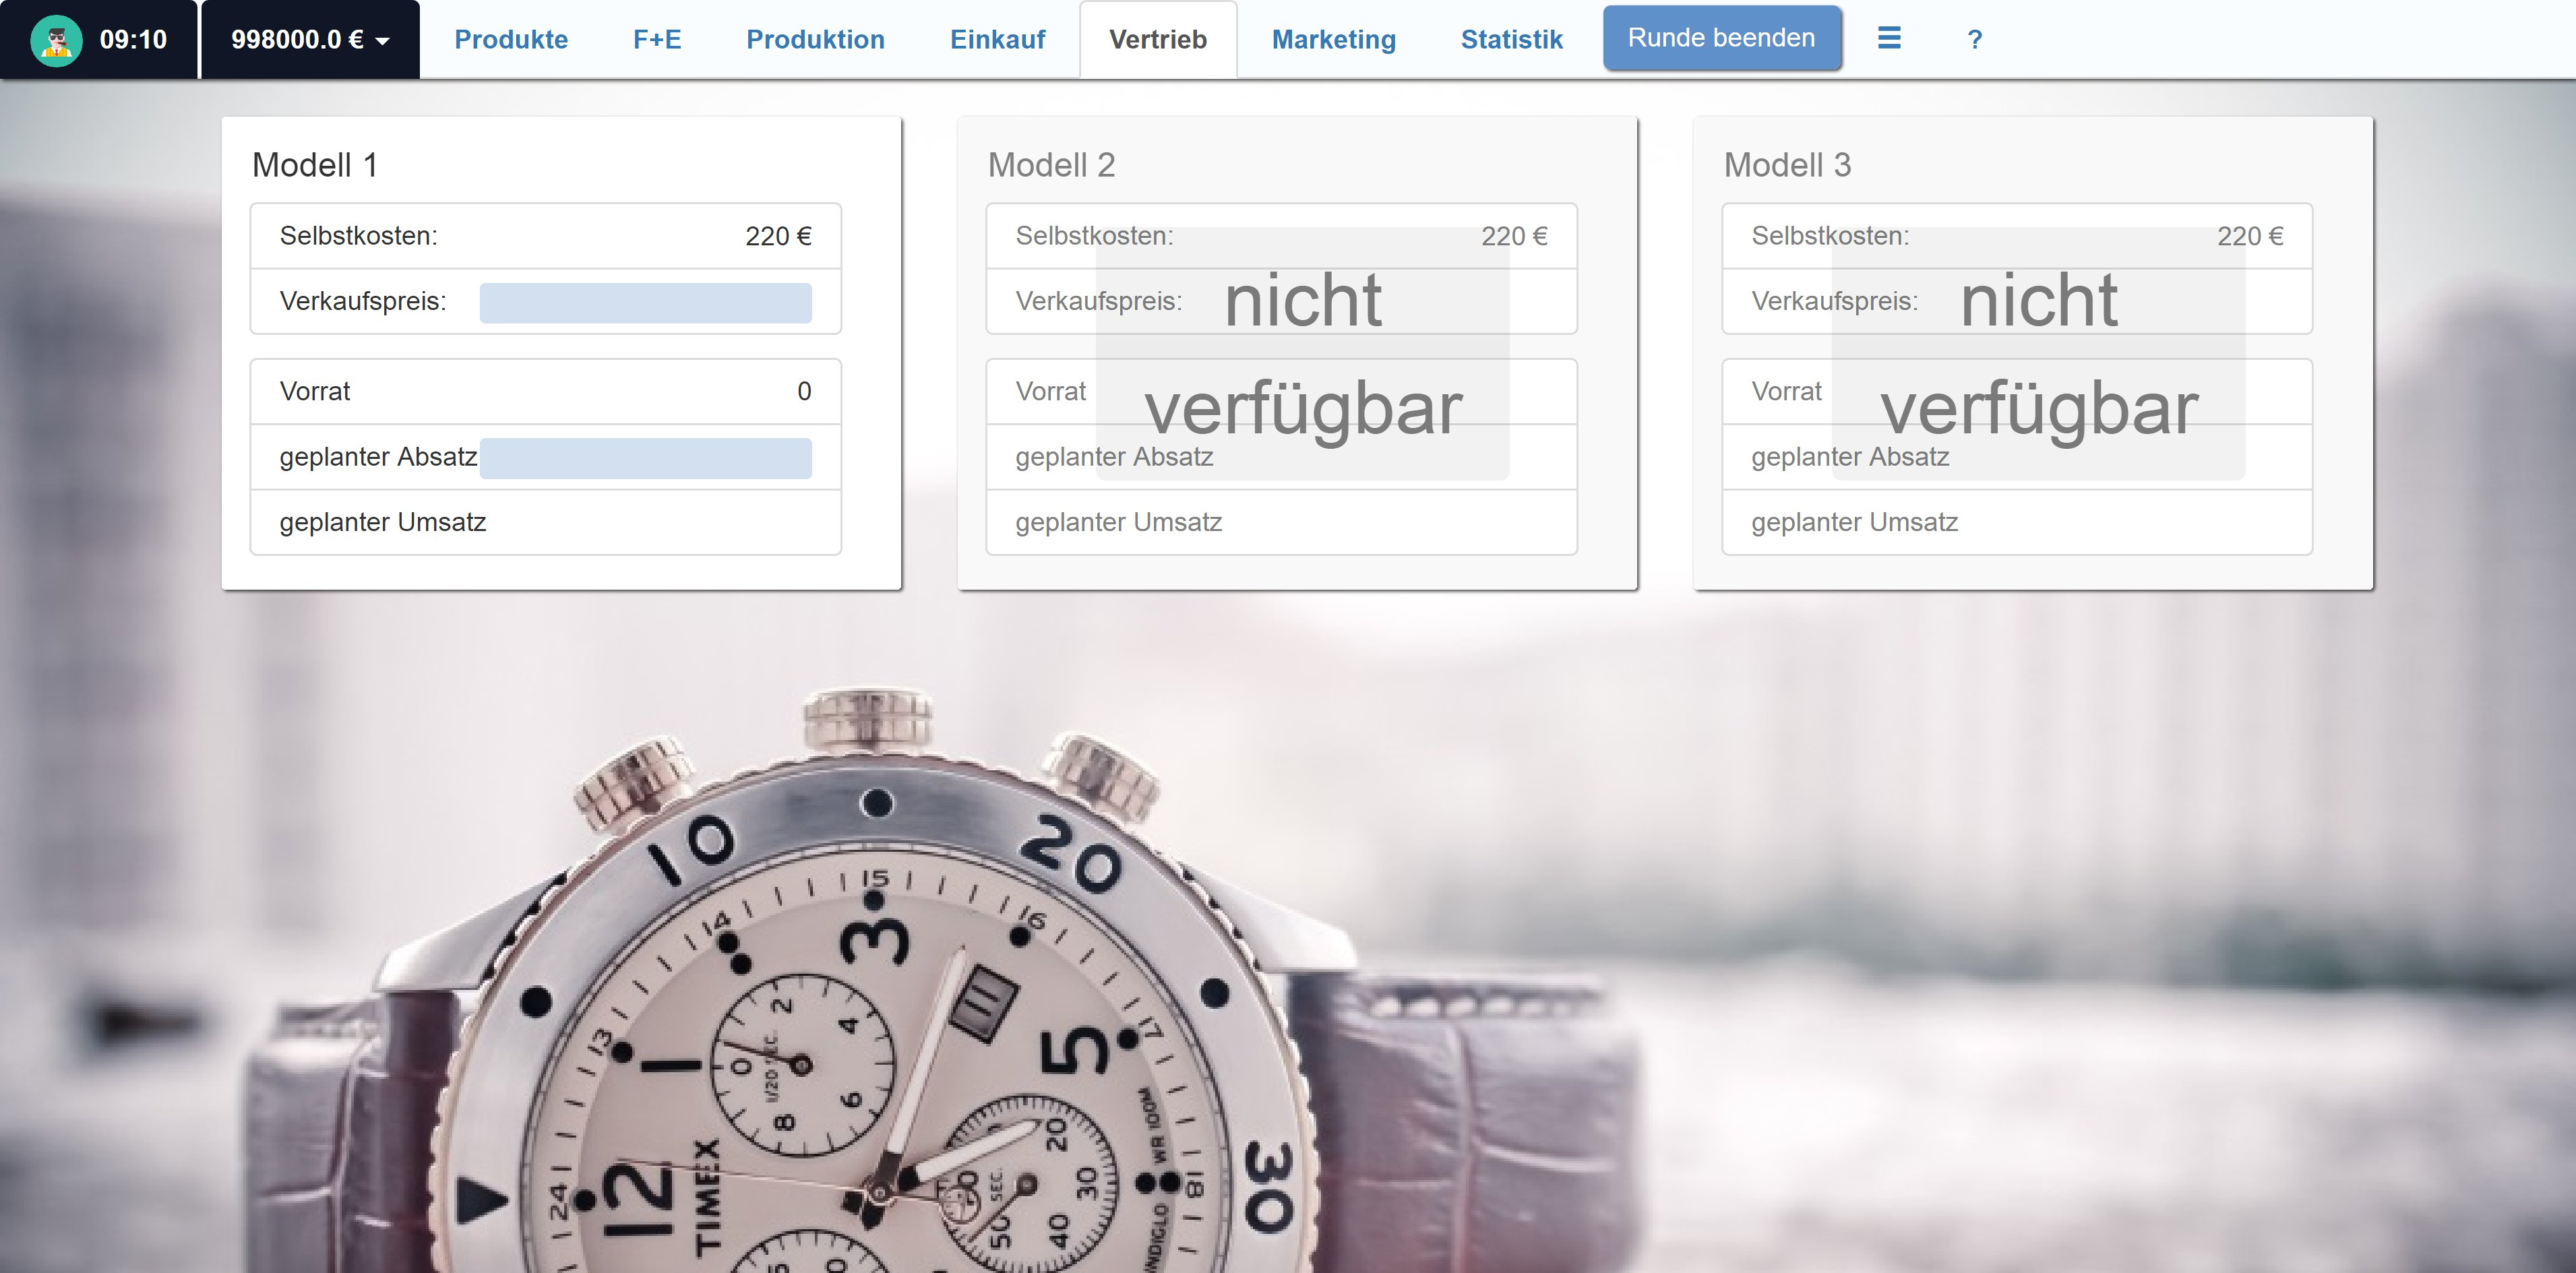
\includegraphics[scale=0.1]{img/bilder_layout/Spiel7.jpg} 
\end{figure}
\begin{figure} [h]
	\centering
	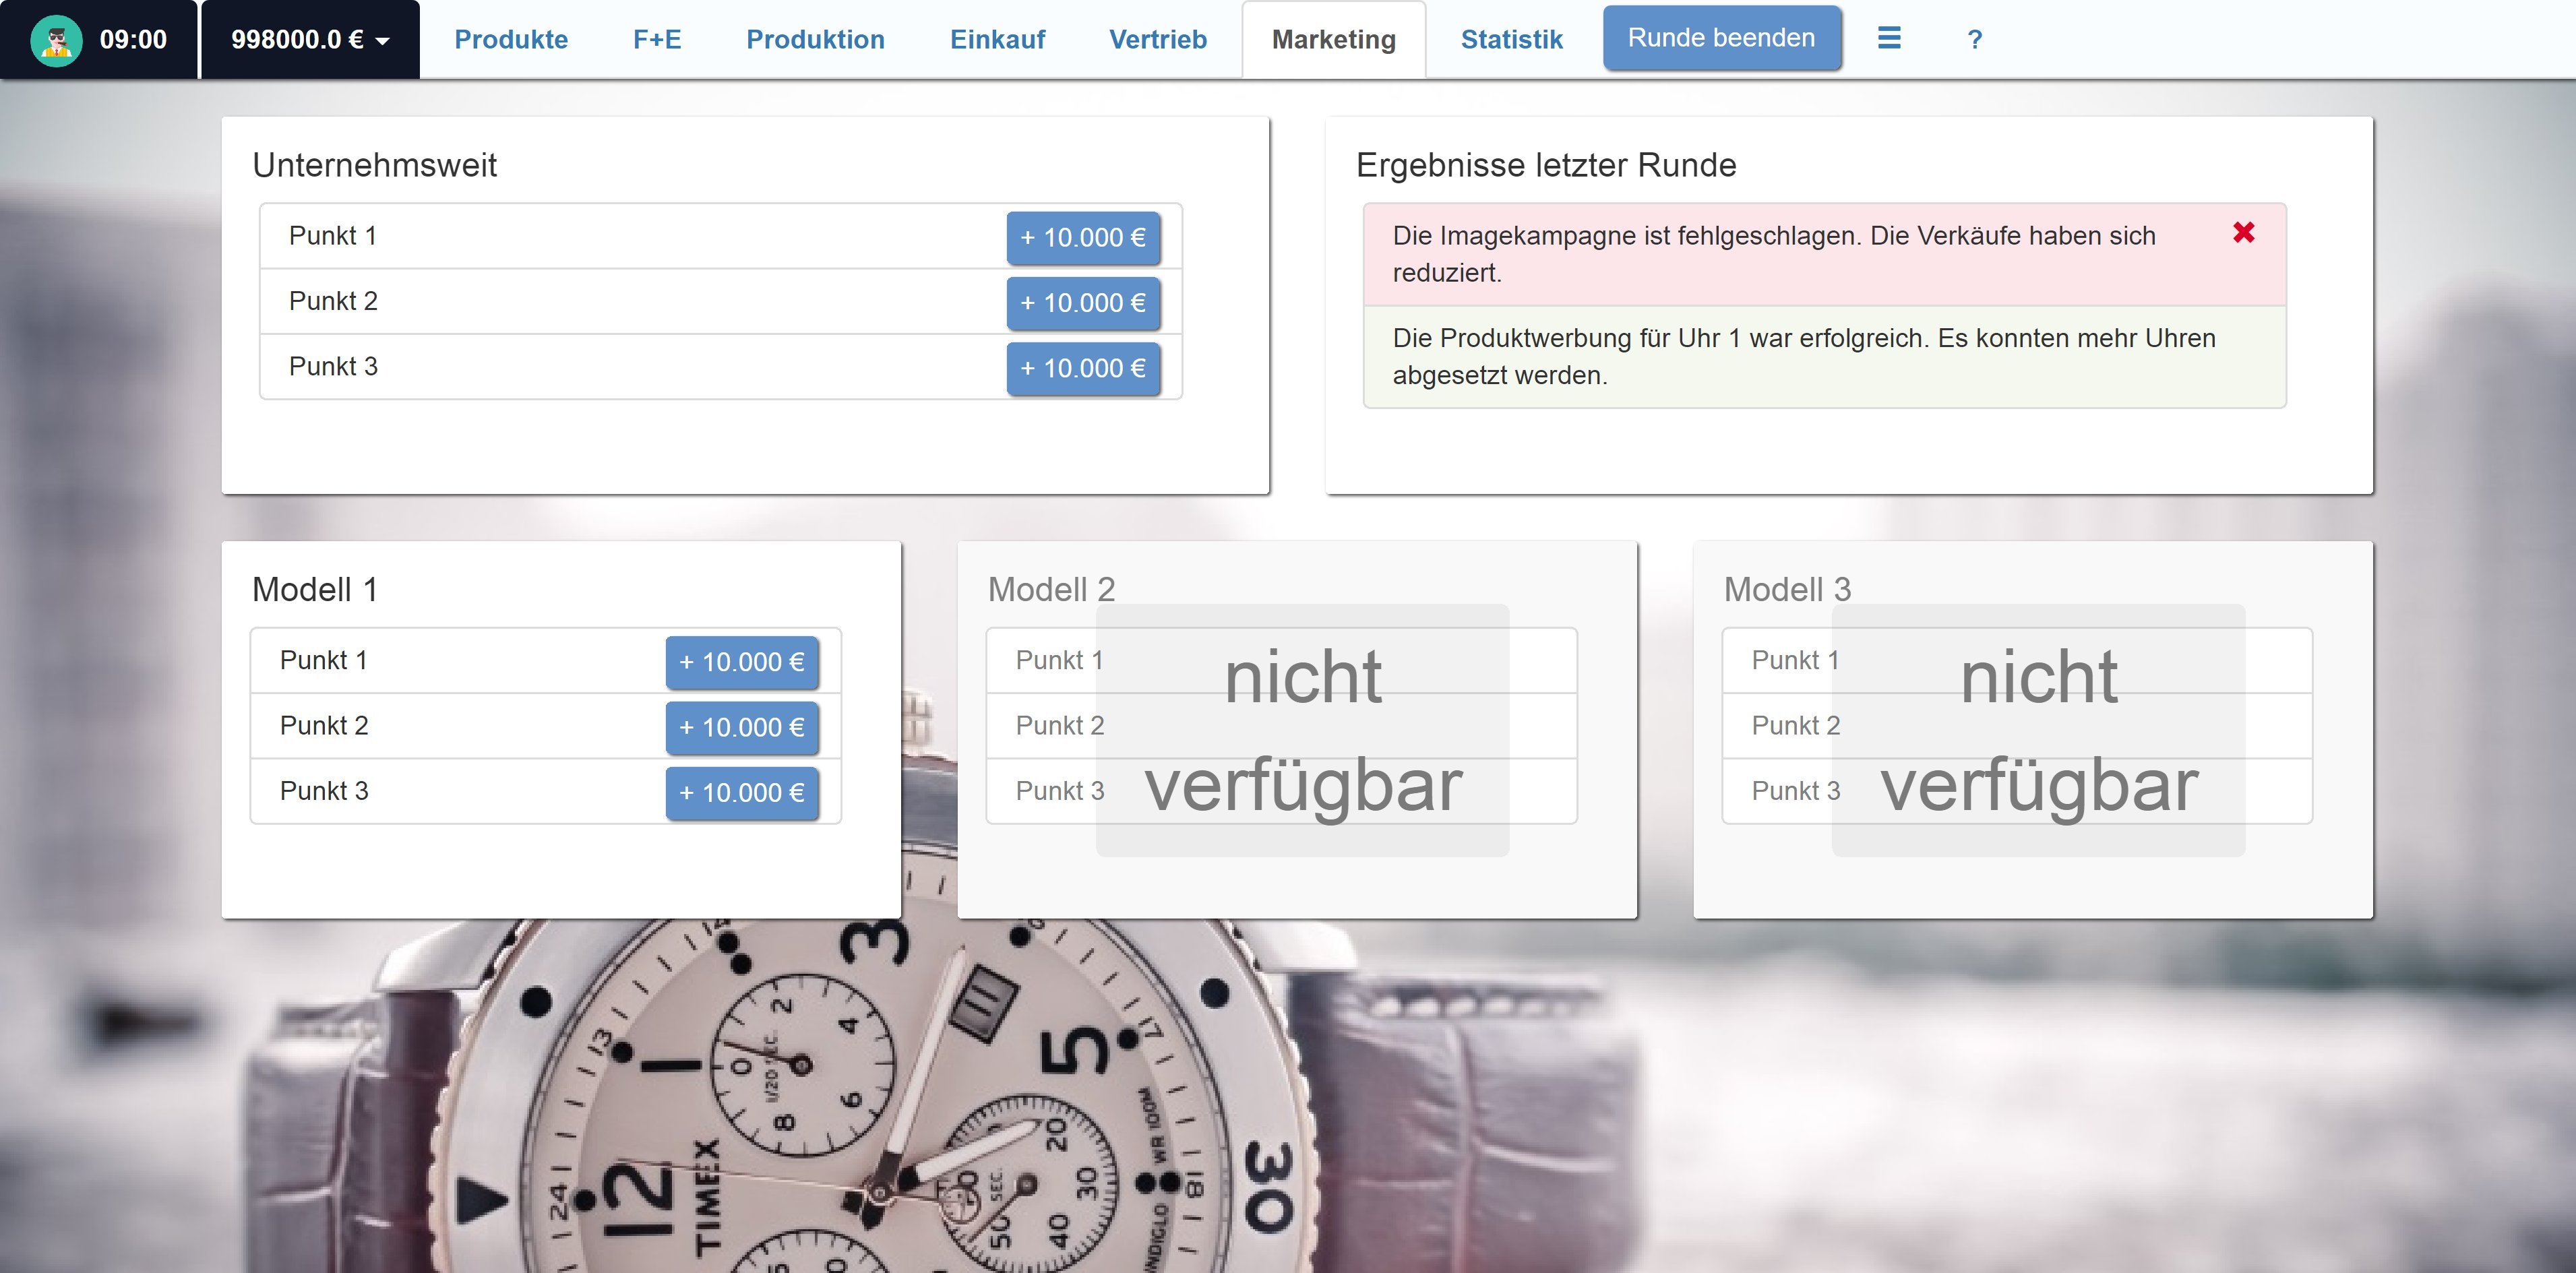
\includegraphics[scale=0.1]{img/bilder_layout/Spiel8.jpg} 
\end{figure}